% XeLaTeX can use any Mac OS X font. See the setromanfont command below.
% Input to XeLaTeX is full Unicode, so Unicode characters can be typed directly into the source.

% The next lines tell TeXShop to typeset with xelatex, and to open and save the source with Unicode encoding.

%!TEX TS-program = xelatex
%!TEX encoding = UTF-8 Unicode

\documentclass[11pt]{article}
\usepackage{geometry,authblk,multicol,amsmath}
\usepackage[square,numbers,sort&compress]{natbib}
\usepackage[textsize=small]{todonotes}                % See geometry.pdf to learn the layout options. There are lots.
\geometry{letterpaper}                   % ... or a4paper or a5paper or ... 
%\geometry{landscape}                % Activate for for rotated page geometry
%\usepackage[parfill]{parskip}    % Activate to begin paragraphs with an empty line rather than an indent
\usepackage{graphicx}
\usepackage{amssymb}
\usepackage{booktabs}
\usepackage{multirow}
\usepackage{url}

% Will Robertson's fontspec.sty can be used to simplify font choices.
% To experiment, open /Applications/Font Book to examine the fonts provided on Mac OS X,
% and change "Hoefler Text" to any of these choices.

%\usepackage{fontspec,xltxtra,xunicode}
%\defaultfontfeatures{Mapping=tex-text}
%\setromanfont[Mapping=tex-text]{Times New Roman}
%\setsansfont[Scale=MatchLowercase,Mapping=tex-text]{Gill Sans}
%\setmonofont[Scale=MatchLowercase]{Andale Mono}

\title{Combinatorial Mixture Models for Single Cell Assays with Application to Vaccine Studies}
\author[1]{Greg Finak}
\author[2]{SC De Rosa}
\author[3]{Mario Roederer}
\author[1]{Raphael Gottardo}

\affil[1]{Vaccine and Infectious Disease Division, Fred Hutchinson Cancer Research Center (FHCRC), Seattle, WA}
\affil[2]{HIV Vaccine Trials Network, Fred Hutchinson Cancer Research Center (FHCRC), Seattle, WA}
\affil[3]{Vaccine Research Center, NIAID, NIH, 40 Convent Drive, Rm 5509, Bethesda, MD 20892}

\date{\today}                                       

\begin{document}
\maketitle

\begin{abstract}
Most biological samples (\textit{e.g.} blood, tissues) are composed of many small and functionally distinct cell subsets that can only be measured accurately using single cell assays. The characterization of these small cell subsets via single cell assays is important and cannot be done with assays that measure cell mixtures. For this reason, an increasingly number of studies rely on single cell assays to provide single-cell measurements of multiple genes and proteins. A common problem in the analysis of such data is to identify, for a given individual, markers (or combinations of markers) that are differentially expressed between two biological conditions (\textit{e.g.}, before/after vaccination), where expression is defined as the proportion of cells expressing that marker (or marker combinations) in the cell subset(s) of interest.
Here we present a Bayesian hierarchical framework based on beta-binomial mixture models for testing for differential marker expression using such single-cell assays. Our model allows inference of differential expression to be subject specific, while borrowing strength across individuals through common prior distributions. We propose two approaches for parameter estimation, one based on an Expectation-Maximization algorithm and one based on Markov chain Monte Carlo. We compare our method against Fisher's exact test, a likelihood ratio test, and basic log-fold changes. Using several experimental immunological based assays measuring proteins and genes at the single-cell level, we find that our method has higher sensitivity and specificity than Fisher's exact test and alternative methods. Using a simulation study we also show that our model is robust from departures from model assumptions. Finally, we also demonstrate how our framework can be extended to testing differential expression of marker combinations using a Dirichlet-Multinomial model. 
\end{abstract}

\section{Introduction}
Cell populations, particularly in the immune system, are never truly homogeneous; individual cells may be in different biochemical states that define functional but measurable differences between them. This single-cell heterogeneity is informative, but lost in assays that measure cell mixtures. For this reason, endpoints in vaccine and immunological studies are measured through a variety of assays that provide single-cell measurements of multiple genes and proteins. In the 1970s, single-cell analysis was revolutionized with the development of fluorescence-based flow cytometry (FCM). Since then, instrumentation and reagent advances have enabled the study of numerous cellular processes via the simultaneous single cell measurement of multiple surface and intracellular markers (up to 17 markers). More recent technological development have drastically extended the capabilities of single-cell cytometry to measure dozens of simultaneous parameters per cell~\citep{Bendall:2011wf}. Although cells sorted using well-established surface markers may appear homogeneous, mRNA expression of other genes within these cells can be heterogeneous4,5 and could further characterize and subset these cells. A new technology based on microfluidic arrays combined with multiplexed polymerase chain reactions (PCR) can now be used to perform thousands of PCRs in a single device, enabling simultaneous, high-throughput gene expression measurements at the single-cell level across hundreds of cells and genes6. While classic gene expression microarrays sum the expression from many individual cells, the intrinsic stochastic nature of biochemical processes results in relatively large cell-to-cell gene expression variability (add references). This heterogeneity may carry important information, thus single cell expression data should not be analyzed in the same fashion as cell-population level data. Special treatment of single cell level data, which preserves information about population heterogeneity, is warranted in general. For this reason, single-cell assays are an important tool in immunology, providing a functional and phenotypic snapshot of the immune system at a given time. These assays typically measure multiple markers simultaneously on individual cells in a heterogeneous mixture such as whole blood or peripheral blood cell mononuclease (PBMC), and are used for immune monitoring of disease, vaccine research, and diagnosis of haematological malignancies~\cite{Altman:1996wf,Betts:2006dw,Inokuma:2007tn}.

During analysis, cell level marker intensities are typically thresholded as positive or negative so that subsets with different multivariate $+/-$ combinations can be obtained as Boolean combinations. For some assays (\textit{e.g.} flow cytometry) such thresholds are set based on prior biological knowledge while for others thresholds are actually given by the assay directly. This is the case for the Fluidigm technology where genes are recorded as absent (not expressed) or present (expressed) at the single cell level. After this thresholding step, we obtain a matrix of Boolean matrix of dimension $N\times K$ where $N$ is the number of cells recorded and $K$ is number of markers. Using this matrix, one can form $2^K$ putative cell subsets; when $K$ is large there is a combinatorial explosion of the number of subsets and many of these might be small or even empty. A common statistical problem is then, for a given marker combination, to identify individuals for whom the proportion of cells expressing that combination is significantly different between two experimental conditions (\textit{e.g.} before and after vaccination). A motivating example from vaccine research is the flow cytometric intracellular cytokine staining (ICS) assay, which is used to identify and quantify individuals' immune responses to a vaccine. Upon vaccination, antigen in the vaccine is taken up and presented to CD4 or CD8 T-cels via antigen presenting cells. While not all T-cells can recognize all antigens, those that recognize antigens in the vaccine become \emph{activated} and produce a variety of cytokines, further promoting the immune response. After activation, this antigen-specific subpopulation proliferates and can persist in the immune system for some time providing \emph{memory} that can more rapidly recognize the same antigen again in the future \cite{McKinstry:2010ei}. These antigen-specific T-cell subpopulations constitute a very small fraction of the total number of CD4 and CD8 T-cells. The ICS assay measures the number of antigen-specific T-cells in PBMC or whole blood by measuring cytokine production in response to activation following stimulation by an antigen that closely matches what was present in the original vaccine. Individual cells are labelled using fluorescently conjugated antibodies against phenotypic markers (CD3, CD4, and CD8), used to subset T-cells, and functional markers (cytokines) used to define antigen specific T-cells~\cite{Horton:2007tsa,DeRosa:2004wp,Betts:2006dw}. A sufficiently large number of cells must be collected to ensure that the rare cell populations can be detected. Subsequently, each individual cell is classified as either positive or negative for each maker based on predetermined thresholds, then the number of cells matching each subpopulation phenotype is counted. These counts are compared between antigen stimulated and unstimulated samples from a individual to identify significant differences. individuals who generate a response after stimulation are called responders whereas individual that do not show any differences are called non-responders. In many single-cell studies, the size of the functionally distinct subpopulations (\textit{i.e.} the number of positive cells) is very low (relative to the total number of cells), and real biological differences might be difficult to detect. Although there is no standard approach to analyzing single-cell assays current methods range from ad-hoc rules based on log-fold changes, to permutation tests based on Hotelling's T$^2$ statistics, to exact tests of 2x2 contingency tables (\textit{e.g.}, Fisher's exact test and $\chi^2$ test\footnote{make sure there is a reference for that. Added ref for the HVTN054 trial and the ICS standardization paper from Horton})~\cite{Trigona:2003,Sinclair:2004hs,Horton:2007tsa,Nason:2006dx,Peiperl:2010ej}. 
All of these methods analyze each individual separately, and no information is shared across individuals even though one could expect some similarities across responders in terms of their response. In addition, these methods generally test one marker at a time or pairwise combinations of markers, raising questions of appropriate multiple testing adjustments, or they perform global tests of significance on multiple markers resulting in decreased power to detect small changes in subsets of cytokines~\cite{Proschan:2009ks,Nason:2006dx}. 

The framework developed in this paper addresses these issues explicitly. In our model, cell counts are modeled via a binomial (or multinomial in the multivariate case) distribution and information is shared across individuals by mean of a prior distribution placed on the unknown proportion(s) of the binomial (or multinomial) likelihood. In order to discriminate between responders and non-responders, the prior is written as a mixture of two Dirichlet distributions where the hyperparameters for each mixture component are shared across individuals. This sharing of information across individuals helps regularize proportion estimates when the cell counts are small, which is typical with single cell assays, and increase sensitivity and specificity to detect responders. Because our framework is multivariate in nature, multiple cell subsets can be model simultaneously, which could help detect some effect biolgical changes spread out across multiple cell subsets~\cite{Nason:2006dx}.

\section{Data structure and notation} 
In this paper we consider two different immunological single-cell assays, one flow cytometry data set and one single-cell gene expression data set.

\textit{Flow cytometry}:
The primary ICS data set is from a  trial testing the GeoVax DNA and MVA vaccines in a prime-boost regimen with 120 individuals (98 vaccines and 20 placebo recipients, see supplementary material~\ref{supp:statpublished}). The goal of this data set was to assess the immune response to the vaccine across multiple stimulations, time points, cytokines and T-cell subsets. Here, we analyze a subset of the data consisting of 98 individual from the vaccinee group at two time points, day 0 and day 182. Samples on day 0 were taken just before vaccination and no response is expected there. The corresponding samples can be used as negative controls. Conversely, day 182 (26 weeks) should be close to the immunogenicity peak, and many individuals are expected to respond, for some cytokines at least. 

\textit{Fluidigm single-cell gene expression}: This is a single-cell gene expression data set of sorted CD8$+$ T-cells from sixteen individuals. T-cells isolated by flow cytometry from sixteen individuals were stimulated in blocks of four individuals with four different antigens (HIV Gag, HIV Nef, CMV pp65 tm10, CMV pp65 nlv5) and gene expression post--stimulation measured at the single-cell level using the BioMark system (Fluidigm) $96 \times 96$ well arrays. The expression from the simulated samples  was compared to paired, unstimulated controls.~\footnote{Add a bit more info here, how many genes, tetramer sorted, etc, Mario et al. could you fill this in?}.


In the remainder of the paper, we use the following notation to describe our model.  From this point on, we assume that we observe cell counts from $I$ individuals in two conditions: stimulated and un-stimulated. Each cell can either be positive or negative for a marker. Given a set of $K$ markers, the measured cells can be classified into $2^K$ positive/negative marker combinations. We denote by $n_{sik}$ and $n_{uik}$, $k=1\dots 2^K$, the observed counts for the $2^K$ combinations in the stimulated and un-stimulated samples. We denote by $N_{si}=\sum_k n_{sik}$ and $N_{ui}=\sum_k n_{uik}$ the total number of cells measured for individual $i$ in each sample. For ease of notations, we will denote by $\mathbf{y}_i$ the vector of observed counts for individual $i$, \textit{i.e.} $\mathbf{y}_{i}=(\mathbf{n}_{si}, \mathbf{n}_{ui})$ where $\mathbf{n}_{si}=\{n_{sik}: k=1,\dots,2^K\}$ and $\mathbf{n}_{ui}=\{n_{uik}: k=1,\dots,2^K\}$. Finally, we define $\mathbf{y}=(\mathbf{y}_1,\dots,\mathbf{y}_I)$.

\section{Differential expression with one marker}
Datasets like the ones presented here are usually analyzed one marker at a times to avoid being underpowered due to the large number of combinations and the potential for very small cell counts in many of the combinations. As a consequence, we first consider the one marker case where cell counts are marginalized and each marker is analyzed separately, \textit{i.e.} $K=1$. In this case, for a given individual, the data can be summarized in a contingency table of $+/-$ cell counts across the un-stimulated and stimulated samples as depicted in Table \ref{tab:twobytwo}.

\begin{table}[ht]
\centering
\parbox{0.8\linewidth}{
\caption{2 x 2 contingency table of counts for marker positive and negative cells between stimulated ($s$) and unstimulated ($u$) conditions for a given individual $i$.}\label{tab:twobytwo}
\centering
\begin{tabular}{rrr}

  \hline
\multicolumn{1}{l}{}&
\multicolumn{2}{c}{Marker}\\
 & Negative & Positive \\ 
  \hline
Stimulated &   $N_{si} - n_{si}$ &   $n_{si}$ \\ 
Unstimulated &   $N_{ui}-n_{ui}$ &   $n_{ui}$ \\ 
   \hline
\end{tabular}
}
\end{table}
For a given individual and stimulation, we consider a marker to be differentially expressed if the proportion of positive cells in the stimulated samples is different from the number of positive cells in the un-stimulated sample. Individuals that show differential expression for a given marker will be called responders for that marker. In this section, we shall be concerned with identifying differential expression one marker at a time, using a beta-binomial mixture model as described in what follows. 

\subsection{Beta-binomial model}
\label{sec:DE}
For a given individual $i$, the positive cell counts for the stimulated and un-stimulated samples are jointly modeled as follows,

\begin{equation}
(n_{si}|p_{si}) \sim \mathrm{Bin}(N_{si},p_{si})\quad \text{and}\quad (n_{ui}|p_{ui}) \sim \mathrm{Bin}(N_{ui},p_{ui})\label{eq:bino_likelihood}
\end{equation}
where $p_{si}$, $p_{ui}$ are the unknown proportions for the stimulated and un-stimulated paired samples. In order to detect responding individuals we consider two competing models:
\begin{equation}
{\cal M}_0: p_{ui}=p_{si}\quad \text{and}\quad {\cal M}_1: p_{ui}\ne p_{si}. \label{eq:beta_prior}
\end{equation}
Under the null model, ${\cal M}_0$, there is no difference between the stimulated and un-stimulated samples, and the proportions are equal. Under the alternative model, ${\cal M}_1$, there is a difference in proportions between the two samples and the individual $i$ is a responder. In some study, such as the ICS trial used here, the proportion of positive cells is expected to only increase after stimulation, in which case the alternative model should be defined as $p_s>p_u$. This alternative parametrization is described in Supplementary Web material.

\subsection{Priors}
Our model shares information across all individuals using exchangeable Beta priors on the unknown proportions, as follows, 
 \begin{align}
(p_{ui} | z_{i}=0)  &\sim \mathrm{Beta}(\alpha_u, \beta_u)\label{eq:prior-null}\\
(p_{si} | z_{i}=1)  &\sim \mathrm{Beta}(\alpha_s,\beta_s) \quad\mathrm{and}\quad (p_{ui}|z_{i}=1) \sim \mathrm{Beta}(\alpha_u, \beta_u) \label{eq:prior-alternative}
 \end{align}
where $z_i$ is an indicator variable equal to one if individual $i$ is a responder, i.e.  ${\cal M}_1$ is true, and zero otherwise, and $\alpha_u, \beta_u, \alpha_s,\beta_s$ are unknown hyper-parameters shared across all individuals. Note that the parameters $\alpha_u, \beta_u$ are explicitly shared across the two models, whereas $\alpha_s,\beta_s$ are only present in the alternative model. Finally, we assume that the $z_i$'s are independent and identically distributed Bernoulli with probability $w$, where $w$ represents the proportion of responders. It follows that marginally, \textit{i.e.} after integrating $z_i$, $p_{ui}$ and $p_{si}$ are jointly distributed as a mixture of a one dimensional and a two dimensional Beta distributions with mixing parameter $w$. Treating the $z_i$'s as missing data, the unknown parameter vector $\boldsymbol\theta\equiv(\alpha_u, \beta_u, \alpha_s,\beta_s, w)$ can be estimated in an Empirical-Bayes fashion using and Expectation-Maximization~\cite{Dempster:1977ul} algorithm as described in Section \ref{sec:estimation}. As an alternative, we also describe a fully Bayesian model where the hyperparameters $\alpha_u, \beta_u$ and $\alpha_s, \beta_s$ are given vague exponential priors with mean $10^3$, and $w$ is assumed to be drawn from a uniform distribution between 0 and 1. In this case, all parameters will be estimated via a Markov Chain Monte Carlo algorithm as described in Section \ref{sec:estimation}. 

\subsection{Parameter estimation}
\label{sec:estimation}
Our estimation algorithms make direct use of the marginal likelihoods, $\mathrm{L}_0$ and $\mathrm{L}_1$, obtained after integrating out the $p_{\{s,u\}i}$'s for the null and alternative models, to simplify our calculations. Given the conjugacy of the priors, the marginal likelihoods $\mathrm{L}_0$ and $\mathrm{L}_1$ are available in closed forms (supplementary material), and are given by,
 \begin{align}
  	\mathrm{L}_0(\alpha_u,\beta_u|\mathbf{y})
	&=\prod_{i=1}^P\binom{N_{ui}}{n_{ui}}\binom{N_{si}}{n_{si}}\frac{\mathrm{B}(n_{si}+n_{ui}+\alpha_u,N_{si}-n_{si}+N_{ui}-n_{ui}+\beta_u)}{\mathrm{B}(\alpha_u,\beta_u)}\label{eq:model1post}
 \end{align} 
and
\begin{align}
	\begin{split}
\mathrm{L}_1(\alpha_u,\beta_u,\alpha_s,\beta_s|\mathbf{y}) 
=\prod_{i=1}^P\binom{N_{ui}}{n_{ui}} \binom{N_{si}}{n_{si}}\frac{\mathrm{B}(n_{ui}+\alpha_u,N_{ui}-n_{ui}+\beta_u)}{\mathrm{B}(\alpha_u,\beta_u)}\frac{\mathrm{B}(n_{si}+\alpha_s,N_{si}-n_{si}+\beta_s)}{\mathrm{B}(\alpha_s,\beta_s)}.\label{model2:unconstrained}
\end{split}
\end{align}
Assuming that the missing data, the $z_i$'s, are known, we define the complete log-likelihood as follows,
\begin{equation}
l(\boldsymbol{\theta}|\mathbf{y},\mathbf{z})=\sum_i z_i l_0(\alpha_u, \beta_u|\mathbf{y}_i) +(1-z_i) l_1(\alpha_u, \beta_u, \alpha_s, \beta_s|\mathbf{y}_i)+z_i\log(w)+(1-z_i)\log(1-w)
\label{eq:cll}
\end{equation}
where $l_0$ and $l_1$ are the log marginal-likelihoods and $\boldsymbol{\theta}\equiv(\alpha_u, \beta_u, \alpha_s,\beta_s, w)$ is the vector of parameters to be estimated. In the one-sided case, the alternative prior specification must satisfy the constraint $p_s>p_u$, and the marginal likelihood derivation involves the calculation of a normalizing constant that is not available in closed form but can easily be estimated. This is described in Supplementary Web material. 

\subsubsection{EM algoritm}
Given an estimate of the model parameter vector $\tilde{\boldsymbol{\theta}}=\left\{\tilde{\alpha}_u,\tilde{\beta}_u,\tilde{\alpha}_s,\tilde{\beta}_s,\tilde{w}\right\}$ and the data $\mathbf{y}$, the E step consists of calculating the posterior probabilities of differential expression, defined by
\[
\tilde z_{i} \equiv \mathrm{Pr}(z_i=1|\mathbf{y},\tilde{\boldsymbol{\theta}})=\frac{\tilde{w} \cdot \mathrm{L}_1(\tilde{\alpha}_u,\tilde{\beta}_u,\tilde{\alpha}_s,\tilde{\beta}_s,|\mathbf{y}_i)}{(1-\tilde{w})\cdot\mathrm{L}_0(\tilde{\alpha}_u,\tilde{\beta}_u|\mathbf{y}_i)+\tilde{w}\cdot\mathrm{L}_1(\tilde{\alpha}_u,\tilde{\beta}_u,\tilde{\alpha}_s,\tilde{\beta}_s|\mathbf{y}_i)}.
\] 
The M-step then consist of optimizing the complete-data log-likelihood over $\boldsymbol{\theta}$ after replacing $z_i$ by $\tilde{z}_{i}$ in \eqref{eq:cll}. Straightforward calculations lead to 
$\tilde w = \sum_i{\tilde{z_i}}/I$, but unfortunately no closed form solutions exist for the remaining parameters. We use numerical optimization as implemented in R's \textit{optim} function to estimate the remaining parameters.  Starting from some initial values, the EM algorithms iterates between the E and M steps until convergence. In our case, we initialize the $z_{i}$'s using Fisher's exact test to assign each observation to either the null or alternative model components. We then use the estimated $z_i$'s to estimate the $p_{ui}$'s and $p_{si}$'s and use these to set the hyper-parameters to their method-of-moments estimates.

\subsubsection{MCMC algorithm}
Realizations were generated from the posterior distribution via MCMC algorithms \citep{Gelfand:1996wc}. All updates were done via Metropolis-Hastings sampling except for the $z_i$'s and $w$ that were done via Gibbs samplings.
Details about the algorithms are given in supplementary material. We used the method of Raftery and Lewis \citep{Raftery:1992vp,Raftery:1996ws} to determine the number of iterations, based on a short pilot run of the sampler. For each dataset presented here, this suggested that a sample of no more than about 1,000,000 iterations with 50,000 burn-in iterations was sufficient to estimate standard posterior quantities. Guided by this, and leaving some margin, we used 2,000,000 iterations after 50,000  burn-ins for each dataset explored here. 


\section{Results}
In this section, we apply our MIMOSA model to the data described in Section, and present the results of a simulation study based on the ICS data.
%The constrained model was applied to an ICS data set from a real--world vaccine trial in order to identify responders to antigen stimulation. The unconstrained model was applied to Fluidigm single--cell gene expression data to identify genes differentially expressed between stimulated and unstimulated conditions in populations of single--cells. We also performed simulation studies to assess the performance of the constrained and unconstrained models in a univariate and multivariate settings.

\subsection{ICS}
\subsubsection*{MIMOSA Outperforms Competing Methods on Vaccine Trial Data from Study HVTN065}

Observations at the day 0 time point were treated as true negatives, while observations at the day 182 time point were treated as true positives (potentially underestimating the sensitivity due to non-responders). We examined the CD4+ T-cell cytokine responses for ENV-1-PTEG and GAG-1-PTEG stimulated samples. An ROC (receiver operator characteristic) analysis was performed to assess the sensitivity and specificity of the constrained MIMOSA model compared to Fisher's exact test, ranked log fold change, and a likelihood ratio test based on the MIMOSA model for identifying vaccine responders and non--responders. 

The MIMOSA model has higher sensitivity and specificity than Fisher's exact test, the likelihood ratio test, or ranked log fold change for discriminating vaccine responders and non--responders when the magnitude of response was small (i.e. ENV-1-PTEG stimulation) (Figure~\ref{fig:HVTN065} A),  (AUC=0.954 for MIMOSA vs. 0.923 for Fisher's exact test vs. 0.827 for LRT vs. 0.775 for ranked fold change). When the magnitude of response was larger (GAG-1-PTEG stimulation), MIMOSA performed as well as Fisher's exact test, and better than other competing methods (Figure~\ref{fig:HVTN065} C) (AUC=0.982 for MIMOSA vs. 0.978 for Fisher's exact test vs. 0.877 for LRT vs. 0.784 for ranked fold change). Irrespective of the magnitude of the response to stimulation, MIMOSA gave better estimates of the observed false discovery rate than competing methods (Figure~\ref{fig:HVTN065} B,D). These results are consistent for other cytokines (see supplementary material~\ref{supp:HVTN065Results}, supplementary figures~\ref{fig:HVTN065Results} and~\ref{fig:HVTN065ResultsCont}).

\subsection{Fluidigm}
\subsubsection{MIMOSA Identifies Stimulation-Specific Patterns of Gene Expression in Fluidigm Single-Cell Data}
We applied the MIMOSA model to Fluidigm single-cell gene expression data from CD8+ T-cells from 16 individuals, under four different stimulation conditions, as well as unstimulated samples. The unconstrained MIMOSA model was fit to each stimulation. From the model we calculated the posterior probabilities of response for each gene, the posterior differences in the proportion of cells expressing each gene between stimulated and unstimulated conditions, as well as the posterior log ratio of the proportion of cells expressing each gene in stimulated and unstimulated conditions. The data are presented in (Figure~\ref{fig:fluidigm} A-C). Importantly, we see that MIMOSA identifies stimulation--specific differences in the proportions of cells expressing each gene, while preserving inter--individual variability (Figure~\ref{fig:fluidigm}). These patterns are evident in the  posterior probabilities (Figure~\ref{fig:fluidigm} A), and preserved in the posterior estimates of the differences of proportions and the posterior log fold changes of proportions (Figure~\ref{fig:fluidigm} B,C). 
 
\subsection{Simulation Studies}

Simulation studies were based on hyper parameter estimates from a dataset is from a phase-I (safety and efficacy) trial of an adenoviral vector vaccine in individuals without prior immunity, measuring four cytokines via intracellular cytokine staining (ICS) in two cell populations from 20 individuals at two time points (zero and 28 days post-vaccination, see supplementary material~\ref{supp:statpublished} for details)~\cite{Peiperl:2010ej}. The statistical analysis of ICS data in the published trial is described in the original manuscript and outlined in the supplementary information (supplementary material~\ref{supp:statpublished})~\cite{Peiperl:2010ej}. The goal of this data set was to assess and quantify response rates of CD4 and CD8 T-cell populations to different antigens.


We examined the performance of the constrained ($p_s>p_u$) and unconstrained ($p_s \ne p_u$) beta--binomial mixture models via simulations. Using hyper parameters estimated from the constrained model fit to data from Gag1--stimulated, CD4--positive, IL2--expressing T--cells from day 28 post--vaccination of the HVTN054 trial~\cite{Peiperl:2010ej}. We simulated data from this constrained model with 500 observations, a response rate of 60\%, an $N$ of 10K, 20K, 30K, 50K, 75K, 100K, and 150K events, with ten independent realizations of data for each $N$. Constrained MIMOSA was fit to this data and the sensitivity and specificity of the model's ability to correctly identify observations from the ``responder'' and ``non--responder'' components was evaluated through analysis of ROC curves, and compared against Fisher's exact test, the likelihood ratio test, and ranked log fold change. This procedure was repeated for the unconstrained model fit to unconstrained data (Figure~\ref{fig:simulations} A-D). The nominal vs observed false discovery rate was also examined to assess the model fit (Figure~\ref{fig:simulations} E-F). 

For both the constrained and unconstrained simulations, MIMOSA out--performed competing methods, including Fisher's exact test, with respect to sensitivity and specificity at all values of $N$ (Figure~\ref{fig:simulations} A, D). Additionally, the false discovery rate for MIMOSA more closely reflected the nominal false discovery rate compared to Fisher's exact test (Figure~\ref{fig:simulations} E, F).
%Since the constrained model relies on Monte--Carlo integration to estimate the normalizing constant in the likelihood calculation, which can be computationally costly, we approximated the.

To assess the sensitivity of the model to deviations from model assumptions, we repeated the simulations with the cell proportions drawn from  truncated normal distributions on $(0,1)$, rather than beta distributions. The means and variances of the truncated normal distributions were set to the maximum likelihood estimates of the beta distributions defined by the $\alpha,\beta$ hyper parameters estimated from the HVTN065 data set (Supplementary Figure~\ref{fig:simulations_trunc}). Even under these departures from the model assumptions, the unconstrained MIMOSA model outperformed Fisher's exact test and performed about as well as the constrained MIMOSA model fit to one-sided data.

\section{Differential expression across marker combinations}
Our beta-binomial model described in section \ref{sec:DE} can be generalized to a Dirichlet-multinomial model to assess differential expression across multiple marker combinations. As described in the data section, we now have counts for each marker combination, denoted by  $\mathbf{n}_{si}=\{n_{sik}: k=1,\dots,2^K\}$ and $\mathbf{n}_{ui}=\{n_{uik}: k=1,\dots,2^K\}$. 
%Table~\ref{tab:multdir} gives an illustration of the counts with two putative markers A and B.
\subsection{Model}

In our multivariate model, the beta distribution is replaced by a multinomial distribution, as follows,
\begin{equation}
 (\mathbf{n}_{ui}|\mathbf{p}_{ui},) \sim \mathcal{M}(N_{ui},\mathbf{p}_{ui})\quad\text{and}\quad (\mathbf{n}_{si}|\mathbf{p}_{si}) \sim \mathcal{M}(N_{si},\mathbf{p}_{si})\label{eq:mult_likeliehood}
 \end{equation}
%; \text{if $i$ is a non--responder}\\
% &(\mathbf{n}_{ui}|\mathbf{p}_{ui}) \sim \mathcal{M}(\mathbf{p}_{ui},N_{ui}); (\mathbf{n}_{si}|\mathbf{p}_{si}) \sim \mathcal{M}(\mathbf{p}_{si},N_{si});\text{if $i$ is a responder}
%\end{align} 
where $N_{\{s,u\}i}=\sum\limits_{k=1}\limits^{2^K} n_{\{s,u\}ik}$ are the number of cells collected and $\mathbf{p}_{ui}$ and $\mathbf{p}_{si}$ are the unknown proportions for the un-stimulated and stimulated samples.

\subsection{Prior}
As in the one-marker case, we share information across individuals using an exchangeable prior on the unknown proportions. This time the beta priors are replaced by Dirichlet priors, as follows,
\begin{align}
(\mathbf{p}_{ui}|z_i=0) &\sim \mathrm{Dir}(\boldsymbol{\alpha}_u)\\\nonumber
(\mathbf{p}_{ui}|z_i=1) &\sim \mathrm{Dir}(\boldsymbol{\alpha}_u) \quad \text{and}\quad (\mathbf{p}_{si}|z_i=1) \sim \mathrm{Dir}(\boldsymbol{\alpha}_s)\label{eq:dir_prior}
\end{align}
where the indicator variable $z_i$ is as defined in \eqref{eq:beta_prior}, i.e. $z_i\sim\mathrm{Be}(w)$ where $w$ is the proportion of responders. As in the beta-binomial case both an EM and MCMC algorithms can be used for parameter estimation. When using a fully Bayesian approach via MCMC, we use the same priors for $\boldsymbol{\alpha}_{\{u,s\}}$ and $w$ as for the beta-binomial model. 

\subsection{Parameter estimation}
Again, to simplify the estimation problem, we make use of the marginal likelihoods that can be obtained in closed forms (see supplementary material). For the null component, the marginal likelihood $\mathrm{L}_0$ is given by,
\begin{align}
\mathrm{L}_0(\boldsymbol{\alpha}_u|\mathbf{n}_s,\mathbf{n}_u) &= \prod_{i=0}^I\frac{ \mathrm{B}(\boldsymbol{\alpha}_{u}+\mathbf{n}_{ui}+\mathbf{n}_{si})}{\mathrm{B}(\boldsymbol{\alpha}_u)} \cdot \frac{N_{si}!}{\prod_k n_{sik}!} \cdot \frac{N_{ui}!}{\prod_k n_{uik}!}
\end{align}
where $\mathrm{B}$ is the $2^K$-dimensional Beta function defined as $\mathrm{B}(\boldsymbol{\alpha})=\prod_k\Gamma(\alpha_k)/\Gamma(\sum_k\alpha_k)$. Similarly the marginal likelihood for the alternative model is given by 
\begin{align}
\mathrm{L}_1(\boldsymbol{\alpha}_u,\boldsymbol{\alpha}_s|\mathbf{n}_s,\mathbf{n}_u) &= \prod_{i=0}^I\frac{\mathrm{B}(\boldsymbol{\alpha}_{u}+\mathbf{n}_{ui}) \mathrm{B}(\boldsymbol{\alpha}_{s}+\mathbf{n}_{si})}{\mathrm{B}(\boldsymbol{\alpha}_s)\mathrm{B}(\boldsymbol{\alpha}_u)} \cdot \frac{N_{si}!}{\prod_k n_{sik}!} \cdot \frac{N_{ui}!}{\prod_k n_{uik}!}.\label{eq:postmult}
\end{align}
The estimation procedures (both EM and MCMC based) for the multinonial-Dirichlet are the same as for the beta-binomial model except that the number of parameters to be estimated is larger. In our experience, the performance of the EM algorithm greatly deteriorates when $K$ becomes larger than 2. The EM algorithms becomes very dependent on the initial values, and can even fail to converge when good initial values are provided. Although our MCMC algorithm is slightly more computational, it does not suffer from this problem and can be used even when $K$ is large. More details about both algorithms are given in supplementary material. 

%\subsection{Parsimonious multivariate model representation}
%In the case of more than two markers, there is a combinatorial explosion in the number of parameters involved in our multinomial-Dirichlet mixture model. The number of parameters to be estimated is $2^{K+1}+1$, which can become very large even for moderate values of $K$. As an example, $K=4$ leads to 33 parameters, and this would require one to have a large number of individuals to properly estimate all parameters. Here, we propose alternative model parametrizations that could be used to address this problem by reducing the number of required parameters. A simple solution would be to assume that the hyper-parameters are constant across marker combinations, \textit{i.e.} $\alpha_{\{s,u\}k}=\alpha_{\{s,u\}}$ for all $k$, and the number of parameters would be reduced to $3$ for any $K$. As attractive as this might sound, such a model would be unrealistic given that certain stimulations are known to induce expression of certain markers more than others. As a more flexible solution, we propose to define $K$ main effect parameters, denoted $\{\theta_k:k=1,\dots,K\}$, for the $K$ markers and represent co-expression parameters as a function of these main effects. So a combination of dregree $l$, with positive markers, $k_1$, $k_2$, \dots, $k_l$ would have a hyperparameter defined as $\tau_l(\theta_{k_1}\theta_{k_2}\cdots\theta_{k_l})^{1/l}$, which is the geometric mean of the corresponding main marker effects scaled by a degree effect, $\tau_l$. Note that the scaling degree effect would be the same for any combinations with the same number of positive markers. The rationale being that as the degree of polyfunctionality increases, the number of cells might decrease (or increase in some instances) and the corresponding parameters should be adjusted by a scaling factor to allow for such variation. The choice of the geometric mean versus an arithmetic mean is to account for the fact that when a particular combination of degree 1 is empty, \textit{i.e.} the corresponding $\theta$ value is close to zero, it is unlikely that other combination involving that maker would be large. Our specification would account for this since the product would be near zero if one of the $\theta$ is near zero.  Finally, the null combination would have a single parameter equal to $\theta_0$.
%
%Assuming that the $\theta$'s and $\tau$'s are stimulation specific, this parametrization would result in $4K+3$ parameters, and would scale linearly with the number of markers providing a good alternative between the fully parametrize model and the model with constant rate for moderate to large values of $K$. In this case, we would recommend the use of an MCMC algorithm. The $\theta$'s would be given the same exponential priors than the unconstrained model, \textit{i.e.} exponentional with mean 100. As for the $\tau's$ we would use an exponential distribution with mean 1\footnote{check with real data to see if that makes sense}. 
%
%\subsection{ICS example with two markers}
%We applied the Multinomial--Dirichlet extension of MIMOSA to the HVTN054 trial data to identify observations with cells expressing polyfunctional cytokine profiles. As a proof of principle we limited the model to the two--component case (Figure~\ref{tab:nesting}), with one component for the null model where we expect no difference between stimulations, and one component for the alternative model where we expect a difference between stimulations. We fit the model to the IL4 and TNFa cytokines for Env3 and Env1 stimulated CD4 T--cells from the day zero and day 28 time points (Figures~\ref{fig:polyfunctionality} and \ref{fig:polyfunctionalityenv1}). 
%
%The day 28 stimulations show that the posterior probability of response is generally higher for the multivariate MIMOSA model than for the univariate models, and the day zero stimulation (Figure~\ref{fig:polyfunctionality}) shows that the multivariate model has fewer false positives than the univariate MIMOSA model fit to distinct cytokine combinations. We compared multivariate MIMOSA against Fisher's exact test. Fisher's exact test was used to test whether the number of cells expressing a specific combination of cytokines (i.e TNFa+/IL4-, TNFa+/IL4+, and so forth) was significantly higher in the stimulated samples than in the unstimulated samples.  In this comparison, Fisher's exact test detected only one of the 8 responders detected by the MIMOSA model in the Env3 stimulated, day 28 data, and detected two false positives in the day zero data. Fisher's exact test also failed to identify four of the 12 responders identified by the MIMOSA model in the day 28, Env1 stimulated data.
%
%

\subsubsection{Polyfunctionality in Fluidigm Single Cell Gene Expression Data}
We fit the multivariate MIMOSA model to the two--sided Fluidigm data, looking at co--expression of pairs of genes in single cells across the four stimulations. In Figure~\ref{fig:polyfunctionality} we show heatmaps of the counts of cells expressing all combinations of the BIRC3 and CCL5 genes in unstimulated and stimulated samples (Figure~\ref{fig:polyfunctionality} A,B). Only CCL5 positive cells express BIRC3, and the expression of BIRC3 increases upon stimulation. The typical approach to analyzing polyfunctional populations from intracellular cytokine staining data (summing the counts over all possible polyfunctional cell populations) would not be appropriate in this case, since changes in the counts of these different cell populations occur in both directions. That is to say, the number of BIRC3-/CCL5+ cells decreases upon stimulation and the number of BIRC3+/CCL5+ cells increases. There is no difference in the marginal counts for any sample (Figure~\ref{fig:polyfunctionality} C). In contrast, multivariate MIMOSA tests all cell subpopulations simultaneously, and identifies a significant difference between stimulated and unstimulated conditions in 13 of the 16 samples (Figure~\ref{fig:polyfunctionality} D). Testing all combinations simultaneously is an advantage over performing multiple univariate tests on the individual combinations, which requires multiplicity adjustment and a potential loss of power. 

Since the Fluidigm data has a limited number of observations (100 cells and 16 samples), we performed simulations (five--dimensional data) to assess the power of the multivariate MIMOSA  model compared to Fisher's exact test on the resulting 2x5 tables, Fisher's exact test performed marginally on each dimension of the data and p--values combined through Fisher's method ($\chi^2=-2\sum_{i=1}^k\log(p_i)$), as well as the likelihood ratio test (Figure~\ref{fig:mvsimulations} A-C). These results show that multivariate MIMOSA has significantly increased power to detect true differences in multivariate data, even with small counts and small effect sizes, and the model is a better fit to the data than other standard approaches tested for analyzing such multivariate count data (Figure~\ref{fig:mvsimulations} B). 

\section{Discussion}
The variety of single--cell assays being adopted by the immunology community is increasing. Flow cytometry, mass cytometry, ELISPOT, Fluidigm, and other single--cell assays can all be analyzed as single--cell count data. Development of effective statistical methods to detect differences in gene or protein expression at the single cell level is becoming increasingly important. Current approaches rely on asymptotic approximations (t--test, or $\chi^2$ test), empirical or ad--hoc methods (2--fold change), or exact tests (Fisher's exact test) where model assumptions are generally not satisfied, all of which can lead to invalid conclusions about the data~\cite{Dittrich:2012bv,Trigona:2003,Sinclair:2004hs,Horton:2007tsa,Proschan:2009ks}. Most importantly, existing classical methods do not share information across samples, resulting in less power to detect true differences than empirical-Bayes and hierarchical modelling approaches, which are widely applied in the microarray literature~\cite{Kendziorski:2003uw,Newton:2001go,Smyth:2005iy}. 

The MIMOSA model presented here uses a mixture model framework of Beta--Binomial or Multinomial--Dirichlet distributions to model counts in experimental units (i.e. individuals) across multiple conditions (i.e. vaccine responders and non--responders). Information is shared across non--responder individuals and across responders individuals through exchangeable Beta or Dirichlet priors, increasing the power to detect true differences between treatment and control conditions compared to Fisher's exact test, even when model assumptions are violated (Figures~\ref{fig:simulations} and Supplementary Figure~\ref{fig:simulations_trunc}). The MIMOSA model based on the Beta--Binomial distribution allows us to constrain the alternative hypothesis to the case $p_s > p_u$, where the proportion of cells in the stimulated sample is strictly greater than the proportion of cells in the matched unstimulated sample. 

Importantly, the analysis of real--world ICS data from vaccine trials demonstrated that the the constrained MIMOSA model performs as well or better than Fisher's exact test or other non-Bayesian alternatives for identifying vaccine responders across multiple antigen stimulations and multiple cytokines (Figure~\ref{fig:HVTN065}). Although the MIMOSA model was fit within each antigen stimulation $\times$ cytokine combination, the model is naive to vaccine time point. Despite this, MIMOSA demonstrated a higher sensitivity and specificity to discriminate between vaccine responders and non-responders on days 0 (pre--vaccination) and 182 (post--vaccination) than the current standard approach (Fisher's exact test), or non--Bayesian alternatives such as the likelihood ratio test or ranking by log--fold change (Figure~\ref{fig:HVTN065} A,C). Our approach treats all day 0 observations as true negatives and all day 182 observations as true positives, yet we know that not all vaccine recipients are likely to exhibit a vaccine response on day 182. None the less, this shortcoming, at worst, leads us to underestimate the true sensitivity of MIMOSA, and does not negatively impact the comparison. Additionally, MIMOSA was found to be a better fit to real--world ICS data from vaccine trials than other analysis approaches, as evidenced by more accurate estimates of true false discovery rate (Figure~\ref{fig:HVTN065} B,D).

Although ICS is the motivating example for the MIMOSA model, it can be applied any type of single--cell assay where cells are dichotomized into positive and negative sets, counted and compared across different conditions. To date, the typical approach to Fluidigm single cell gene expression analysis has been focused on identifying differences in the continuous part of the signal, corresponding to the $C_t$ values and the ``missing'' data from cells that don't express a given gene has generally been ignored, or used as part of ad--hoc pre-filtering\cite{Flatz:2011jb}. The ability of MIMOSA to identify stimulation--specific expression patterns in single--cell gene expression data demonstrates not only the broader utility of the method, but importantly, also demonstrates that biologically relevant signal is present in the proportion of cells expressing each gene under different conditions (Figure~\ref{fig:fluidigm} A-C). MIMOSA explicitly models and performs inference on the observed positive cell counts between different conditions. Additionally, extending the model to take into account multiple  conditions is straightforward. 

Detecting differences in polyfunctional cell populations (i.e. identifying changes in cell populations that co--express multiple proteins, cytokines, or genes), is important in vaccine research, since it allows the identification of more precisely defined, more homogeneous cell popualtions~\cite{Milush:2009bz}. These polyfunctional cell populations may be correlated with differential vaccine response or efficacy and have the potential to inform vaccine development and trial design. What's more, changes in these polyfunctional cell populations are not always detectable when looking at the marginal populations (Figure~\ref{fig:polyfunctionality} A-C). Existing methods for identifying polyfunctional cytokine profiles from ICS data either separately test individual combinations of cytokines, or perform global tests between groups of individuals even when the populations under study are known to be heterogeneous (i.e. mixtures of responders and non--responders).  Sometimes these tests are entirely empirical in nature (i.e. thresholds based on fold change or some factor over background), and these methods generally do not share information across observations~\cite{Dittrich:2012bv,Trigona:2003,Sinclair:2004hs,Horton:2007tsa,Proschan:2009ks,Nason:2006dx}. As others have pointed out, in order to have the most power to detect a true difference, the statistical test should be selected taking into account the cytokine combinations of interest~\cite{Nason:2006dx}. Here we have shown that MIMOSA has higher sensitivity and specificity than these competing methods to identify true differences between conditions in multivariate count data (Figure~\ref{fig:polyfunctionality} A, and Figure~\ref{fig:mvsimulations} A,C), and the model generally provides a better fit to the single--cell assay count data arising from studies with these types of experimental designs (Figure~\ref{fig:mvsimulations} B).

\section{Conclusions}
We have developed a mixture model framework that we call MIMOSA .for identifying differences between treatment conditions in paired observations of cell counts from a variety of single--cell assays that frequently arise in the context of vaccine trials and immunological studies. Our model can be applied in a univariate or multivariate fashion, and we have shown that it has greater sensitivity and specificity than other typical approaches used to analyze the type of count--based data derived from single cell assays, including Fisher's exact test, the non-Bayesian likelihood ratio test, or ad--hoc rank based approaches. The software is implemented in R and C++, and is freely available from GitHub (\url{http://www.github.org/finak/MIMOSA}). 



%\subsection*{Statistical Analysis of Responder and Non--responder Calls for Direct Comparison Against the Bayesian Mixture Model Approach}
%Positivity calls for vaccine responders and non--responders depend upon the selection of an appropriate threshold. Therefore, to compare different methods of analysis, comparable thresholds for positivity must be selected for the methods. Our mixture modelling approach is fit within each stimulation, and we make positivity calls based on a false discovery rate calculated across individuals, within each stimulation, whereas the originally published analysis makes multiple testing adjustments within individuals, across cytokines. In order to have comparable response rates, we reanalyzed the ICS data using Fisher's one--sided exact test (as described in the original publication) but made positivity calls based on the false discovery rate computed across individuals within each stimulation.
%
%Our approach to modelling an individual's response to vaccine using ICS data takes a Bayesian approach. We model all observations (individuals) simultaneously for each combination of cytokine and stimulation (including the unstimulated samples). For a given cytokine, we let $n_s$ be the number of cytokine--positive cells in the stimulated sample, $N_s$ the total number of cells in the stimulated sample, and $n_u, N_u$, the number of cytokine--positive and total number of cells in the unstimulated sample, respectively. Note that usually, $N_u \ne N_s$. The observed count data $\mathbf{y}$ is a matrix of size $4 \times P$, where $P$ is the number of participants. For the $i$'th individual $\mathbf{y}_i = \left<N_{si},n_{si},N_{ui},n_{ui}\right>$, and can be represented as the following contingency table: 
% latex table generated in R 2.14.0 by xtable 1.5-6 package
% Wed Oct 12 09:41:50 2011

%\subsection{The Mixture of Beta--Binomials}
%Although we have specified the two models for the data, we do not know which observation was generated by which model. Clearly, not all individuals are expected to exhibit an immune response to a stimulation. Any individual observation, $y_i$, could either be generated by model~\eqref{eq:null} or by model~\eqref{eq:alternate}. We capture this uncertainty with a mixture framework of the two competing beta--binomial models. The likelihood for the mixture is given by:

%The classification of responder and non--responder individuals was compared between the multivariate MIMOSA model, univariate MIMOSA models applied to each cytokine combination, and Fisher's exact test applied to each cytokine combination. 

%The multivariate MIMOSA model detected two additional responders than Fisher's exact test at the 1\% FDR level (Table~\ref{tab:MDFisher}, top left). The univariate MIMOSA model applied to each cytokine combination individually also outperformed Fisher's exact test, detecting one more responder for the IL4 and TNFa combination (Table~\ref{tab:MDFisher} bottom right), and two more responders for the TNFa and not IL4 cytokine combination (Table~\ref{tab:MDFisher} bottom left).  In the multivariate case, the two responders detected by MIMOSA that were missed by Fisher's exact test had a  2.4--fold and 2.5--fold increase in the proportion of TNFa+/IL4- cells in the stimulated samples than the unstimulated samples. These are the same two samples detected by the univariate MIMOSA model for TNFa+/IL4- cells, one of which also exhibits a 1.7--fold increase in IL4+/TNFa- expression between stimulated and unstimulated samples that was detected by univariate MIMOSA, but not detected by Fisher's exact test.
%

\begin{figure}[htbp] %  figure placement: here, top, bottom, or page
   \centering
%   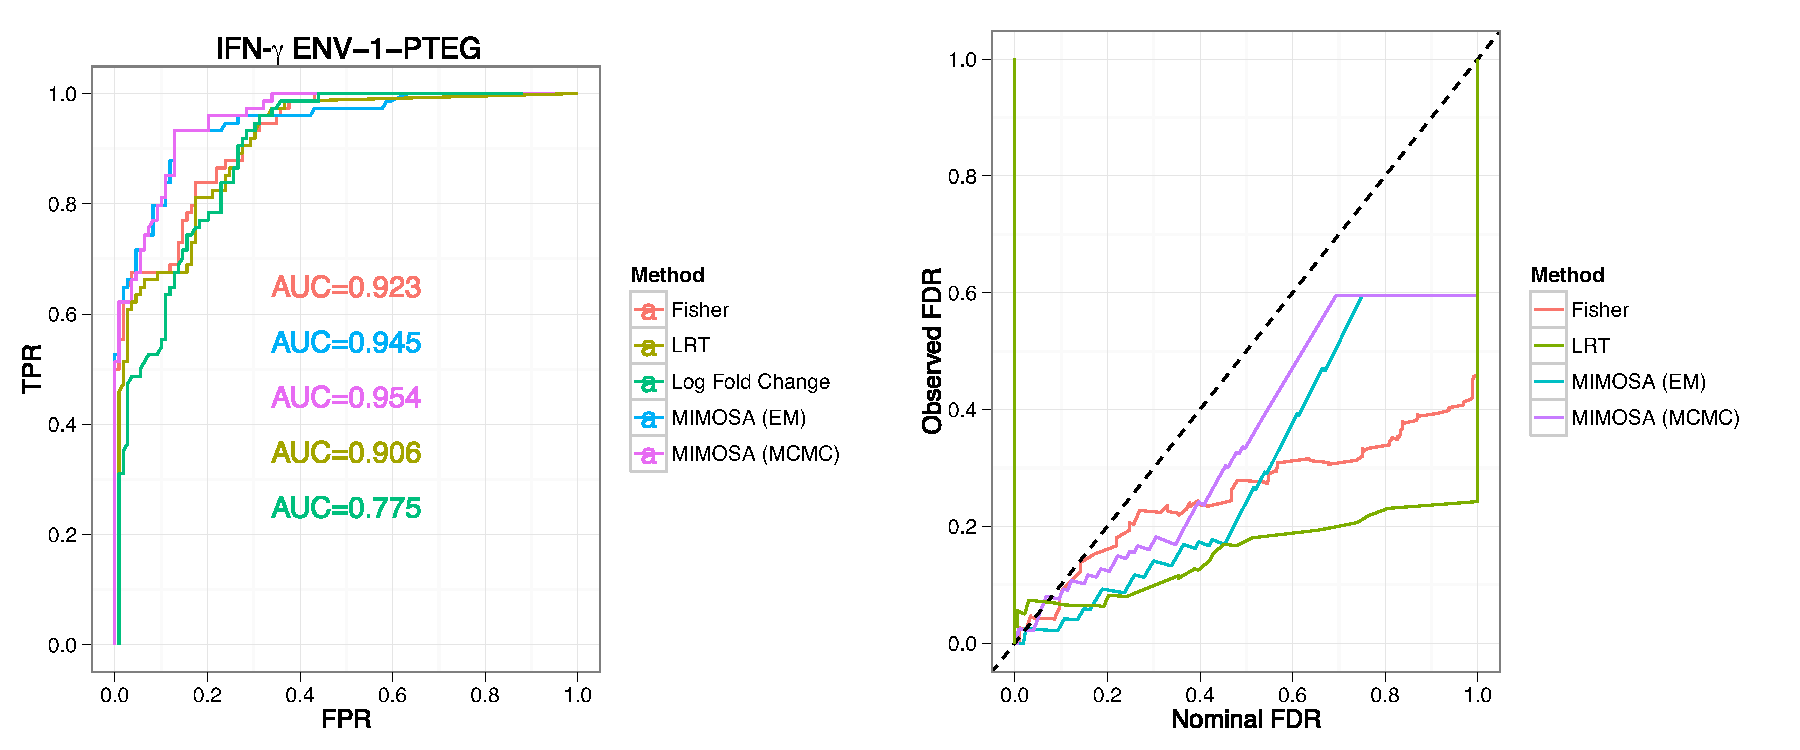
\includegraphics[width=.75\columnwidth]{Figures/2}\\ 
%   \includegraphics[width=.75\columnwidth]{Figures/12} 
\begin{tikzpicture}
    \node[anchor=south west,inner sep=0] at (0,0) {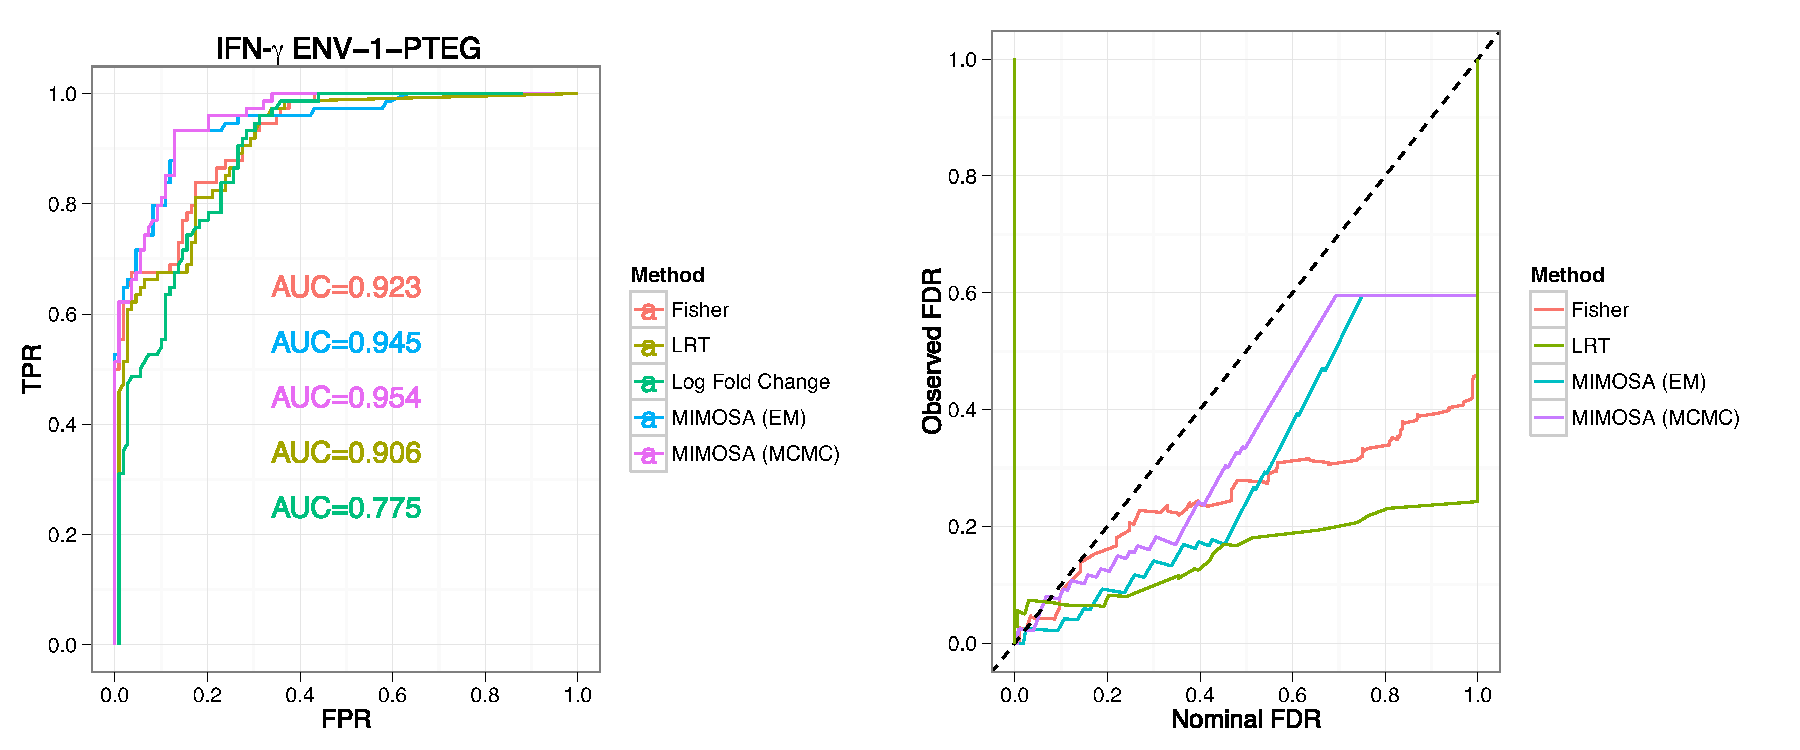
\includegraphics[width=.6\columnwidth]{Figures/2}};
    \node[anchor=south west, inner sep=0] at (0,-3.75){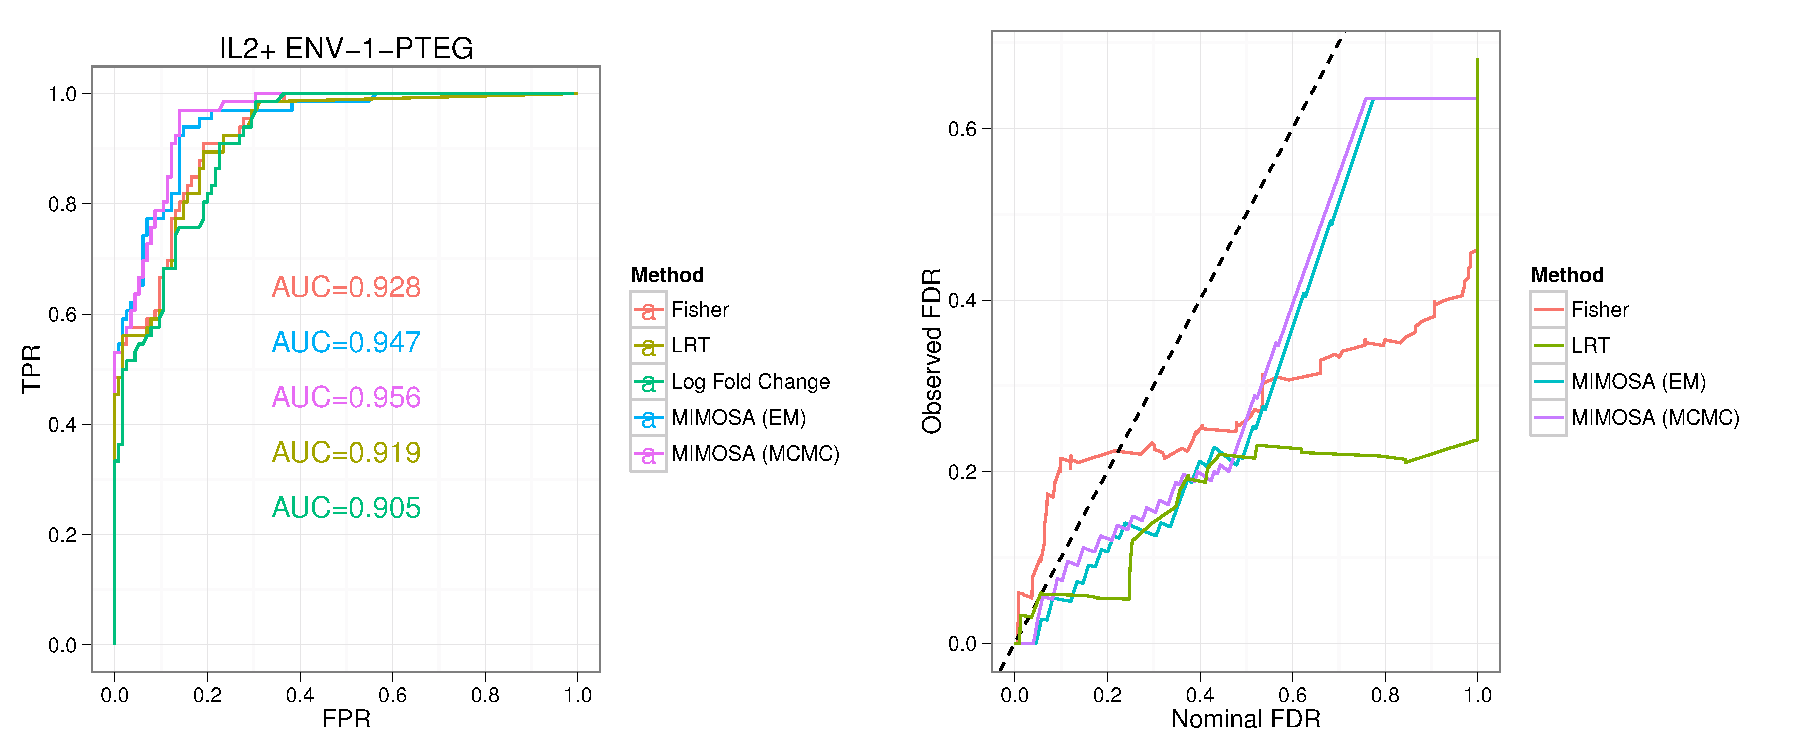
\includegraphics[width=.6\columnwidth]{Figures/1}};
    \node at (0,3.4) [font=\tiny\sffamily] {A} ;
    \node at (4.6,3.4) [font=\tiny\sffamily] {B} ;
    \node at (0,-0.25) [font=\tiny\sffamily] {C} ;
    \node at (4.6,-0.25) [font=\tiny\sffamily] {D} ;
\end{tikzpicture}
   \caption{Performance of MIMOSA (EM and MCMC implementations, one--sided model) and competing methods on ICS data from HVTN065. Sensitivity and specificity (ROC analysis) as well as observed and nominal false discovery rates for positivity calls from CD4+ T--cells stimulated with A--B) ENV-1-PTEG and expressing IFNg or C--D) ENV-1-PTEG and expressing IL2. ROC and FDR plots of other cytokine combinations can be found in the supplementary material.}
\label{fig:HVTN065}
\end{figure}

%   \caption{Performance of the constrained and unconstrained Beta--binomial mixture model vs Fisher's exact test on simulated data. Data were simulated from a constrained model with hyper--parameters estimated from a real data set of Gag1 stimulated, CD4+, IL2 expressing T--cells on day 28 from the HVTN054 trial. For total cell counts from 10,000 to 150,000, we simulated ten data sets each of 500 observations with a response rate of 40\%. The performance, measured by the AUC (area under the curve), of the constrained and unconstrained Beta--binomial mixture model compared to Fisher's exact test is shown in the first panel, as a function of increasing number of cells. The beta distributions for the estimated and true hyper parameters are shown in the second panel for one simulated data set, with N=150,000 events. The ROC curve for Fisher's exact test and the constrained and unconstrained Beta--binomial model for the same simulation are shown in the third panel. The observed vs expected false discovery rate for Fisher's exact test and the constrained and unconstrained Beta--binomial model are shown in the fourth panel.}
%   \label{fig:simulations}

\begin{figure}[htbp]
\centering
\begin{tikzpicture}
\node[anchor=south west, inner sep=0] at (0,0) {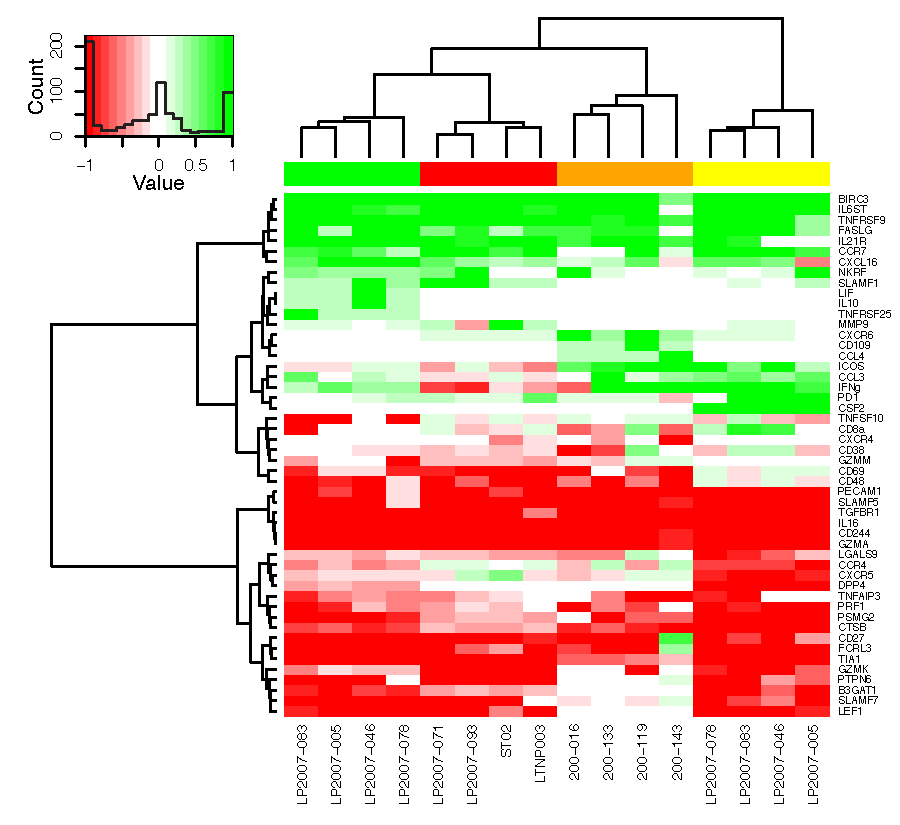
\includegraphics[width=0.29\columnwidth]{Figures/Fluidigm_plot1.pdf}};
\node[anchor=south west, inner sep=0] at (4.6,0) {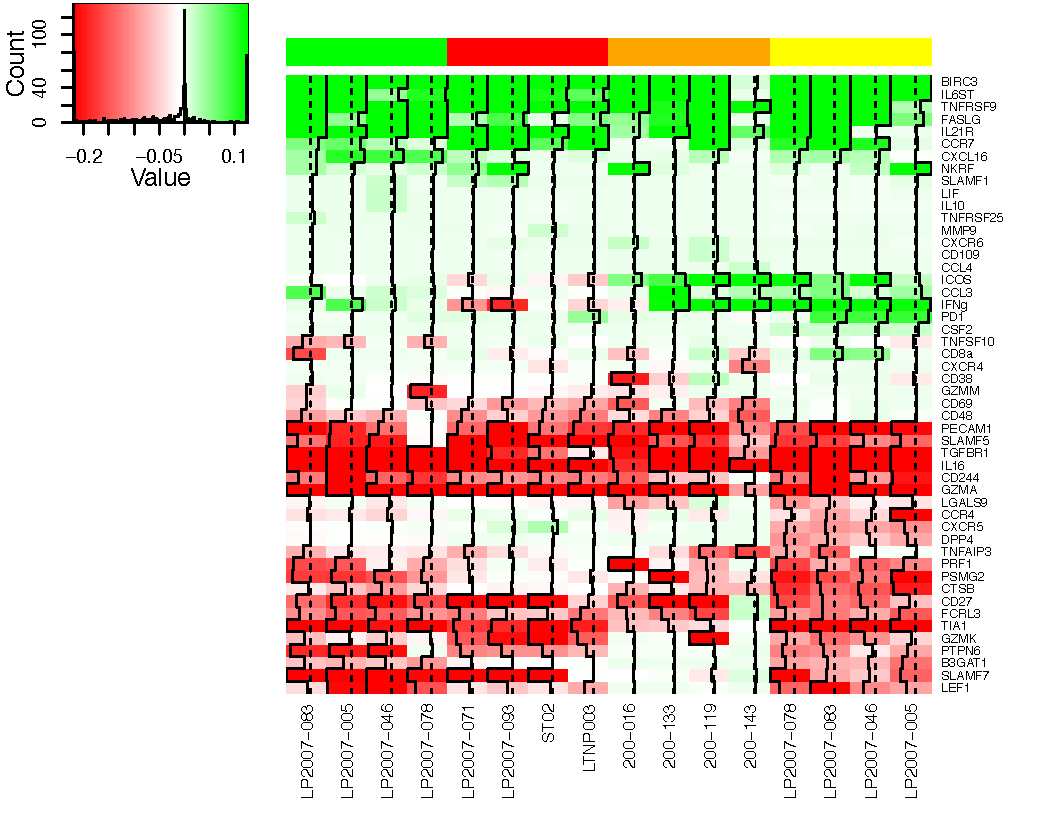
\includegraphics[width=0.29\columnwidth]{Figures/Fluidigm_plot2.pdf}};
\node[anchor=south west, inner sep=0] at (9.1,0) {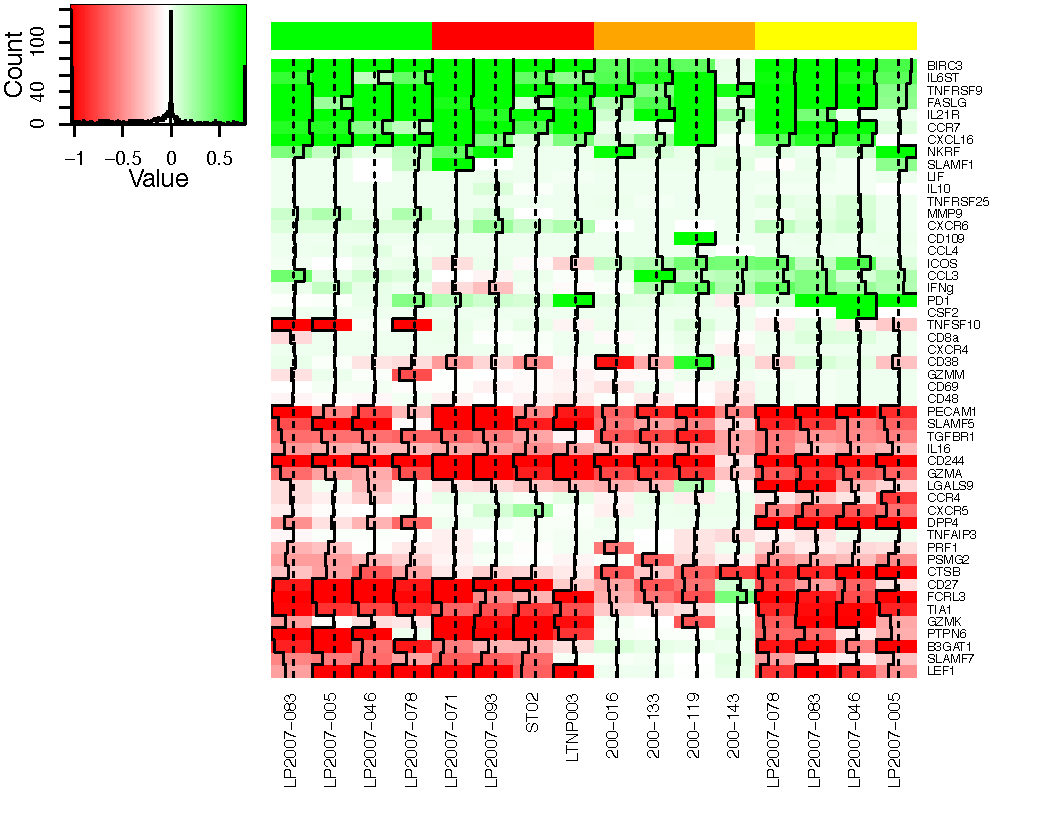
\includegraphics[width=0.29\columnwidth]{Figures/Fluidigm_plot3.pdf}};
\node at (0,3) [font=\tiny\sffamily] {A} ;
\node at (4.5,3) [font=\tiny\sffamily] {B} ;
\node at (8.95,3) [font=\tiny\sffamily] {C} ;
\end{tikzpicture}
\caption{Signed posterior probability, difference and log-odds ratio of the proportion of single cells expressing each gene on a 96x96 Fluidigm array. The posterior probability of response times the sign of the change in expression is shown in A) (red indicates a significant decrease, green a significant increase, relative to the control). Columns and rows are clustered based on these signed posterior probabilities. B) The $log_2$ ratio of the proportion of cells expressing a gene in the stimulated vs. control samples. Rows and columns are ordered as in A) for comparison. C) The difference in the proportion of cells expressing each gene in the stimulated vs. control samples. Ordering of the rows and columns is preserved as in A). The traces show the deviations of each cell from zero. Colors along the columns denote different stimulations (green: CMV pp65 nlv5, red: HIV Gag, orange: HIV Nef, yellow: CMV pp65 tm10).}

\label{fig:fluidigm}
\end{figure}


\begin{figure}[htbp] %  figure placement: here, top, bottom, or page
   \centering
\begin{tikzpicture}
    \node[anchor=south west,inner sep=0] at (0,0) {\includegraphics[width=.4\columnwidth]{Figures/Sim_onesided_ROC_5000.pdf}};
    \node[anchor=south west, inner sep=0] at (6,0){\includegraphics[width=0.4\columnwidth]{Figures/Sim_onesided_FDR_5000.pdf}};
    \node at (0,3.4) [font=\tiny\sffamily] {A} ;
    \node at (4.6,3.4) [font=\tiny\sffamily] {B} ;
\end{tikzpicture}
   \caption{Comparison of positivity detection methods on data simulated from the one--sided model. Ten simulations were generated at an $N$ of 5,000 total counts using hyper--parameter estimates from real ICS data (IFNg expressing CD4+ T--cells stimulated with ENV-1-PTEG from HVTN065) with a five--fold effect size between responder and non--responder components. A) Average ROC curve over the 10 simulated data sets (N=5,000) D) Average observed and nominal false discovery rate over 10 simulated data sets (N=5,000). Curves are shown for MIMOSA (one--sided), Fisher's exact test, the likelihood ratio test, and ranked log fold--change. Results for the two--sided model and the MIMOSA fit to a model violating model assumptions, as well as other values of N are in the Supplementary Material.}\label{fig:simulations}
\end{figure}

\begin{figure}[htbp]
\centering
\begin{tikzpicture}
\node[anchor=south west, inner sep=0] at (0,0) {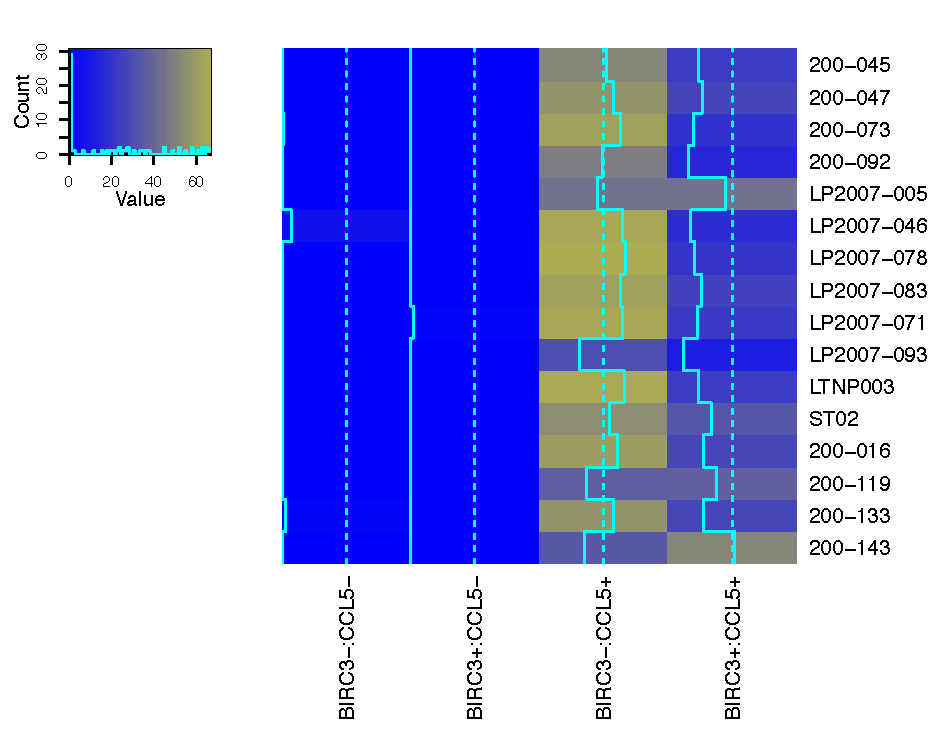
\includegraphics[width=0.4\columnwidth]{Figures/Fluidigm_Multivariate_BIRC3_CCL5_Unstim_Counts.pdf}};
\node[anchor=south west, inner sep=0] at (6.5,0) {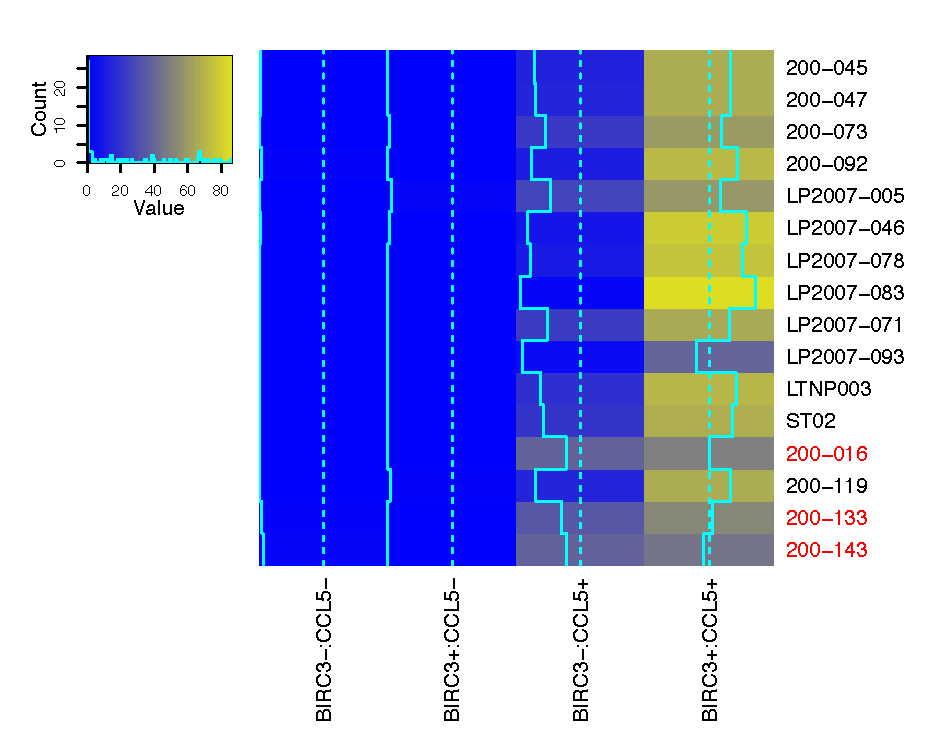
\includegraphics[width=0.4\columnwidth]{Figures/Fluidigm_Multivariate_BIRC3_CCL5_Stim_Counts.pdf}};
\node [anchor = south west, inner sep=0] at (0,-4) {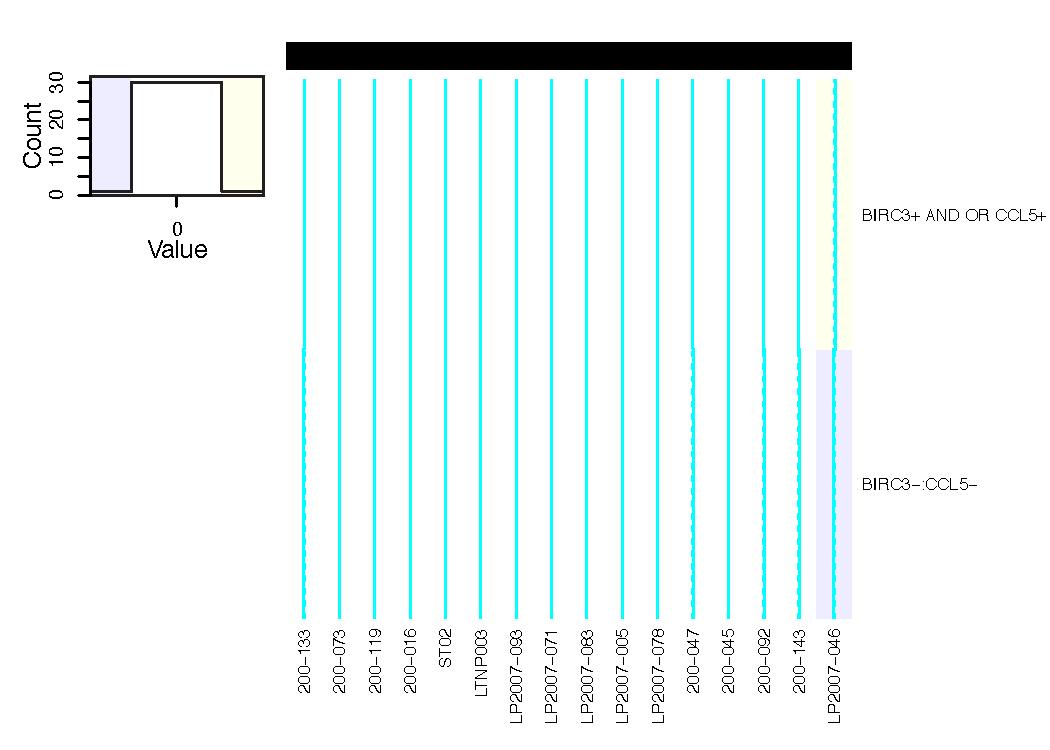
\includegraphics[width=0.4\columnwidth]{Figures/Fluidigm_Multivariate_Marginalized_BIRC3_CCL5.pdf}};
\node [anchor=south west, inner sep=0] at (6.5,-4) {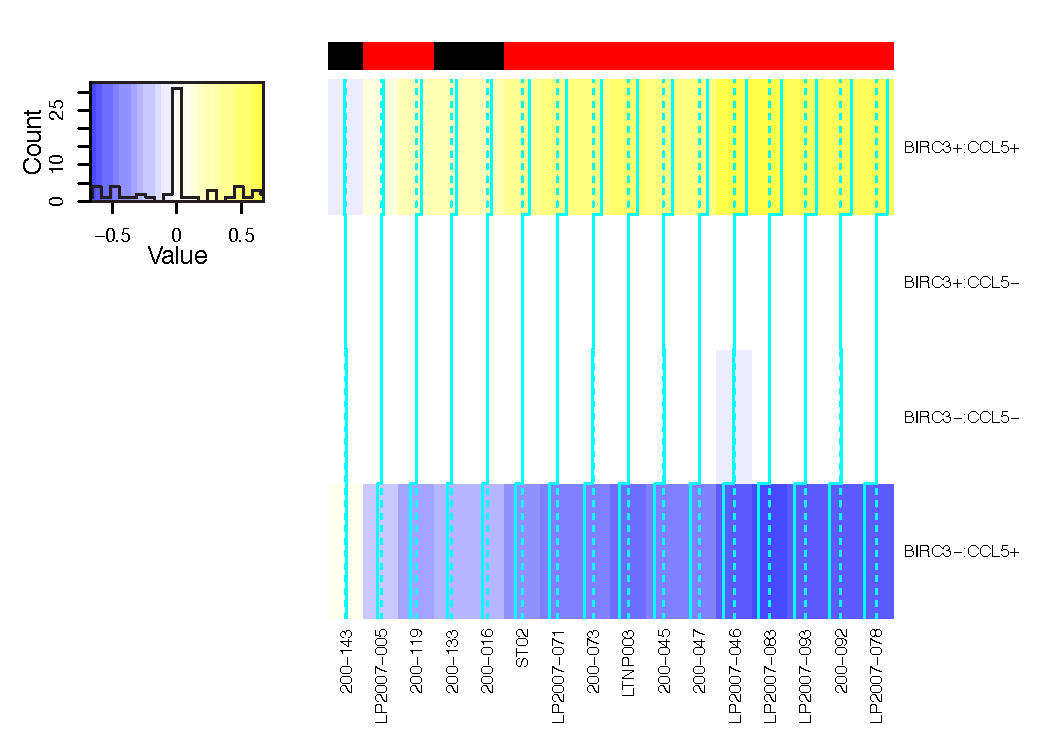
\includegraphics[width=0.4\columnwidth]{Figures/Fluidigm_Multivariate_BIRC3_CCL5.pdf}};
\node at (0,4.5) [font=\tiny\sffamily] {A} ;
\node at (6.25,4.5) [font=\tiny\sffamily] {B} ;
\node at (0,0) [font=\tiny\sffamily] {C} ;
\node at (6.25,0) [font=\tiny\sffamily] {D} ;
\end{tikzpicture}
\caption{Counts of cells expressing different combinations of BIRC3 and CCL5 genes in the A) unstimulated and B) stimulated conditions. The posterior difference in proportions between stimulated and unstimulated samples fitting the C) marginalized counts D) multivariate combinations. No difference is observed from the marginalized counts, while multivariate MIMOSA detects a difference between stimulated and unstimulated conditions in 13 of 16 samples.}
\label{fig:polyfunctionality}
\end{figure}

\begin{figure}[htbp] %  figure placement: here, top, bottom, or page
   \centering
\begin{tikzpicture}
    \node[anchor=south west, inner sep=0] at (0,0){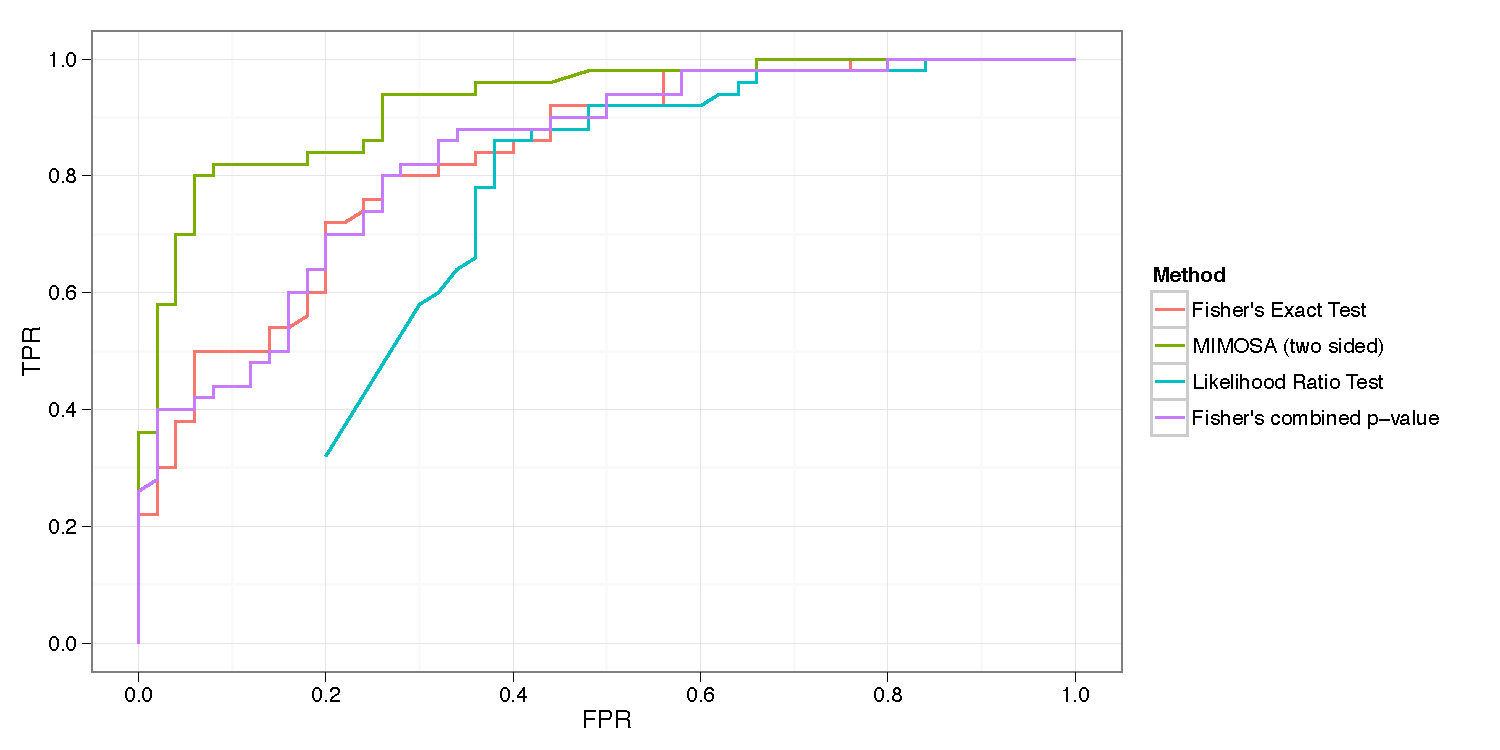
\includegraphics[width=0.4\columnwidth]{Figures/Multivariate_Sims_ROC.pdf}};
   \node[anchor=south west, inner sep=0] at (6,0) {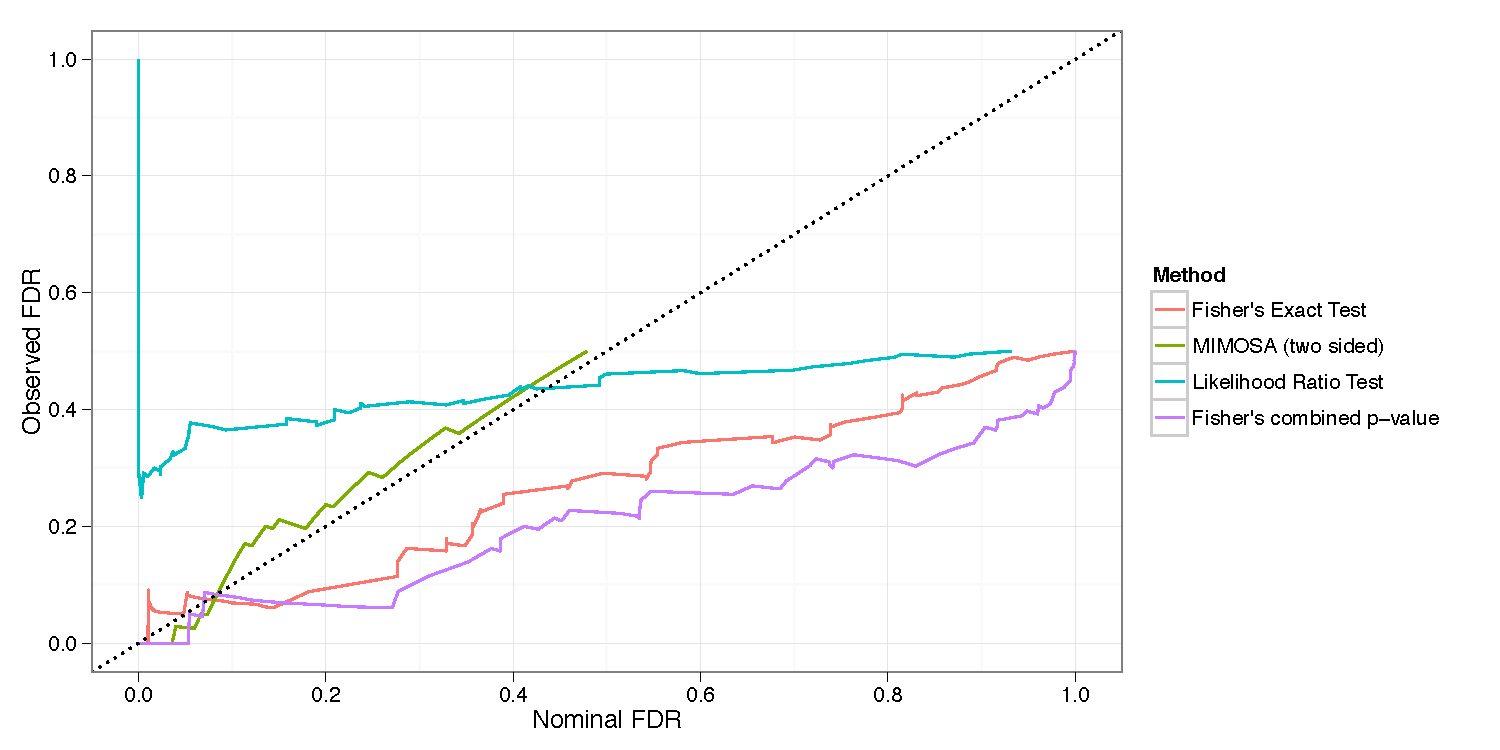
\includegraphics[width=0.4\columnwidth]{Figures/Multivariate_Sims_FDR.pdf}};
    \node at (0,3.5) [font=\tiny\sffamily] {A} ;
    \node at (6,3.5) [font=\tiny\sffamily] {B} ;
\end{tikzpicture}
   \caption{Multivariate simulations from a two--sided model. Ten, eight-dimensional data sets were simulated from a two--sided model with an effect sizes of $2.5\times 10^{-3}$ and $-2.5\times 10^{-3}$ in two of the eight dimensions (N=1,500). Multivariate MIMOSA was compared against Fisher's exact test, the likelihood ratio test, and Fisher's combined p--value (combining Fisher's exact test run marginally on each of the five dimensions). A) Average ROC curves for the competing methods over 10 simulations. B) Average observed and nominal false discovery rate for each method over 10 simulations.}
   \label{fig:mvsimulations}
\end{figure}
\clearpage
%
%\begin{figure}[htbp] %  figure placement: here, top, bottom, or page
%   \centering
%   \includegraphics[width=4in]{Figures/simulations_violatedmodel} 
%   \caption{Sensitivity to departures from model assumptions. We generated data from a variant of the constrained model ($p_s>p_u$) where the proportions were simulated from truncated normal distributions on $(0,1)$, rather than from beta distributions. The mean and variance of the normal distributions was given by $\mu=\alpha/(\alpha+beta), \sigma^2=(\alpha\beta)/((\alpha+beta)^2(\alpha+\beta+1))$, where $\alpha,\beta$ are the Beta--prior hyper parameters for the MIMOSA model estimated from real data ($s, u$ subscripts omitted for brevity). The AUC for the unconstrained MIMOSA model and Fisher's exact test as a function of event count are shown in the first panel. The beta distributions for the estimated and true hyper parameters  are shown in the second panel. The ROC curves for one data set and the observed and true false discovery rates for the model and Fisher's exact test are shown in the third and fourth panels.}
%   \label{fig:simulations_trunc}
%\end{figure}


%\begin{figure}[htbp] %  figure placement: here, top, bottom, or page
%   \centering
%   \includegraphics[width=6in]{Figures/PositivityRates} 
%   \caption{Comparison of MIMOSA and Fisher's exact test for calling responders in ICS data. Response rates for IL2 and IFNg cytokine positivity in Gag2 and Pol2 stimulated samples at days 0 and 28 in the CD4 and CD8 T--cell subpopulations of the HVTN054 ICS data. In the treatment groups, response rates for the MIMOSA model are greater than or equal to those for Fisher's exact test at day 28 but are equal (and zero) at day 0 as expected. In the control groups, response rates are equal (and zero) between Fisher's exact test and the MIMOSA model at day 0 and at day 28, as expected.}
%   \label{fig:positivityrates}
%\end{figure}

%\begin{figure}[htbp] %  figure placement: here, top, bottom, or page
%   \centering
%   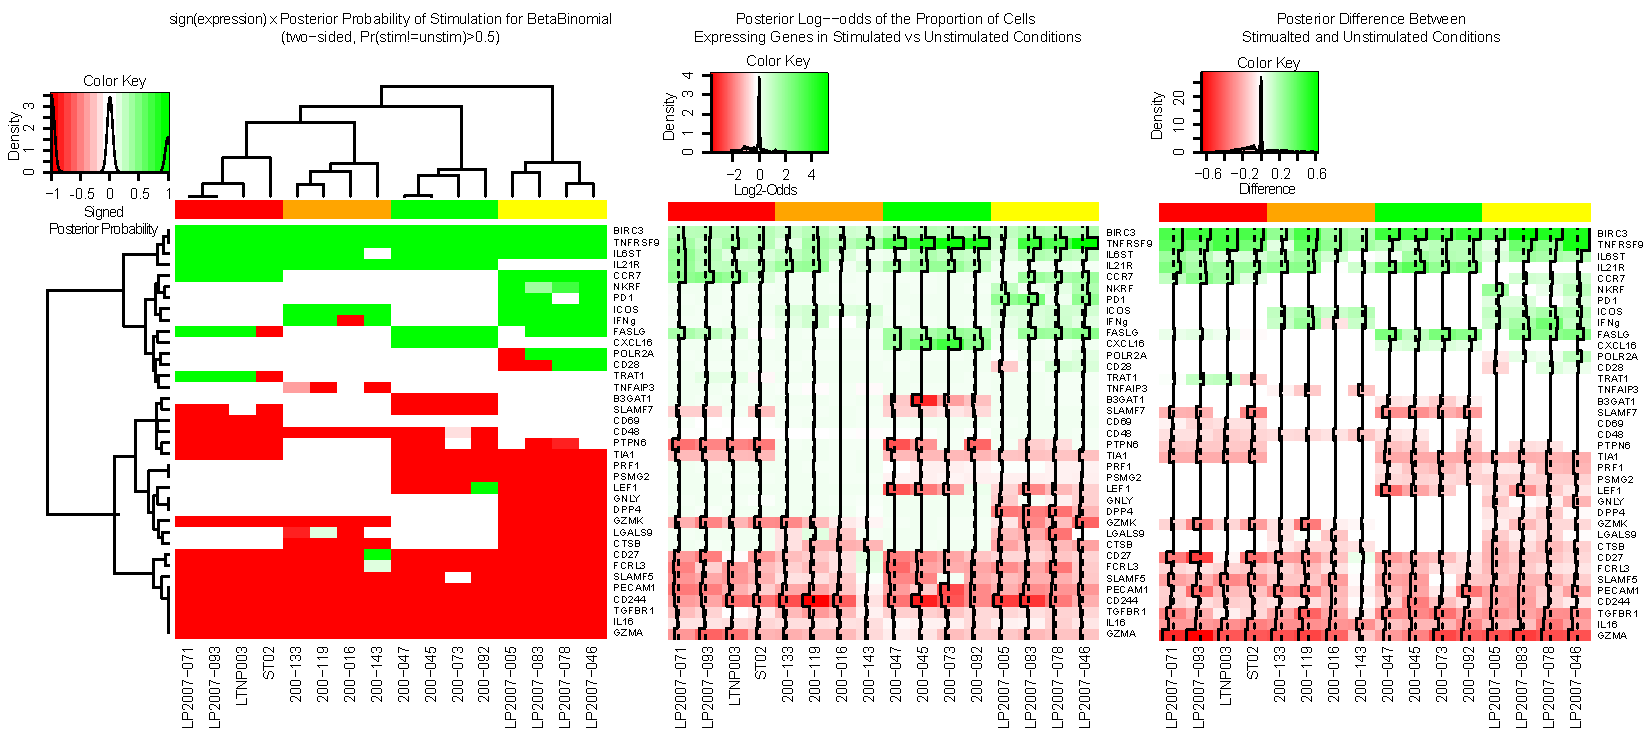
\includegraphics[width=6in]{Figures/FluidigmMIMOSA.pdf} 
%  % \caption{Likelihood surface and volcano plot for IFNg producing, CD4+ T-cells in Gag2 stimulated vs control samples on day 28. A significant difference between control and stimulated samples is called at the 1\% FDR threshold (red) for the Beta--binomial model, and at 1\% for FDR adjusted p--values from Fisher's exact test (green). The likelihood surface shows the observed counts from stimulated and unstimulated samples. The volcano plot shows the difference between the proportion of cytokine positive cells in the stimulated and unstimulated samples, for the maximum likelihood estimates of the proportions (triangles) and for the MAP estimates (crosses). The effect of shrinking the MAP estimates towards zero can be seen in the volcano plot.}
%%   \label{fig:icsdata}
%\caption{Signed posterior probability, difference and log-odds ratio of the proportion of single cells expressing each gene on a 96x96 Fluidigm array. The posterior probability of response times the sign of the change in expression is shown in the first panel (red indicates a significant decrease, green a significant increase, relative to the control). Columns and rows are clustered based on these signed posterior probabilities. The middle panel shows the $log_2$ odds ratio of the proportion of cells expressing a gene in the stimulated vs. control samples. Rows and columns are ordered as in the left panel for comparison. The right panel shows the difference in the proportion of cells expressing each gene in the stimulated vs. control samples. Ordering of the rows and columns is preserved as in the first panel. The traces show the deviations of each cell from zero.}
%\label{fig:fluidigm}
%\end{figure}

%\begin{figure}[htbp] %  figure placement: here, top, bottom, or page
%   \centering
%   \includegraphics[width=6in]{Figures/Polyfunctionality_ggplot2} 
%   \caption{Posterior probabilities from the four--dimensional, Multivariate--Dirichlet, MIMOSA model, compared against posterior probabilities from univariate MIMOSA for each combination of the cytokines IL4 and TNFa, on days zero and 28 for Env--2 peptide stimulated CD4+ T--cells.}
%   \label{fig:polyfunctionality}
%\end{figure}
%
%\begin{figure}[htbp] %  figure placement: here, top, bottom, or page
%   \centering
%   \includegraphics[width=6in]{Figures/Polyfunctionality_Env1} 
%   \caption{Posterior probabilities from the four--dimensional, Multivariate--Dirichlet, MIMOSA model, compared against posterior probabilities from univariate MIMOSA for each combination of the cytokines IL4 and TNFa, on days zero and 28 for Env--1 peptide stimulated CD4+ T--cells.}
%   \label{fig:polyfunctionalityenv1}
%\end{figure}
%

\renewcommand{\thesection}{S.\arabic{section}}
\renewcommand{\thesubsection}{\thesection.\arabic{subsection}}
\setcounter{section}{1}
\setcounter{subsection}{0}
\renewcommand{\figurename}{Supplementary Figure}
\setcounter{figure}{0}
%\todo[inline]{Note that the Supplementary Information section needs corrections to notation and overall}

\section*{Supplementary Information}
\subsection{HVTN065 and HVTN054 Vaccine Trial ICS Data Description}
\label{supp:statpublished}
HVTN065 is a phase 1 (safety and immunogenicity) trial of GeoVax HIV/AIDS DNA and MVA vaccine in 120 individuals (100 vaccinees, 20 placebo recipients, parts A and B). CD4 and CD8 T--cell epitope specific immune responses were measured via the ICS assay. Other humoral and cellular immune responses were measured via ELISA, and neutralizing antibody assays. Cytokines measured in the ICS assay included IFNg, TNFa, IL2, and IL4, and antigens included three Env, three Gag, and three Pol peptide pools. Results of the trial have been published~\citep{Goonetilleke:2006jk}.

HVTN054 is a phase 1 (safety and immunogenicity) trial of an adenoviral vector vaccine in individuals without prior immunity~\cite{Peiperl:2010ej}. The vaccine vector expressed Gag, Pol and Env proteins from multiple HIV clades~\cite{Peiperl:2010ej}. Vaccine was given at two increasing doses, as well as a placebo. T--cell responses to antigens in the vaccine were measured via the ICS assay~\cite{Peiperl:2010ej,Horton:2007tsa}. The cytokines measured were IFNg (Interferon--$\gamma$), IL2 (Interleukin--2), TNFa (Tumor necrosis factor--$\alpha$) and IL4 (Interleukin 4)~\cite{Horton:2007tsa}. The sample size consisted of 20 vaccine and four placebo recipients. The original statistical analysis of the positivity calls is described in the associated publication~\cite{Peiperl:2010ej}. The Gag stimulated, IL2 expressing, CD4+ T--cell data from day 28 was used to derive hyper--parameter estimates for the simulation studies. 

\subsection{Constrained Beta--binomial model}
\label{supp:constrained}
We can define a model where we constrain the stimulated proportions under the alternative model such that $p_s>p_u$. In this case, the only changes required are for the alternative marginal likelihood $\mathrm{L}_1$ defined in equation~\eqref{model2:unconstrained}. The marginal likelihood for the constrained model becomes $\mathrm{L}_1\times \mathrm{C}$, where $\mathrm{C}$ is a ratio of normalizing constants for the likelihood and the prior.

\begin{align}
\begin{split}
	 \mathrm{C}=\frac{\int\limits_{p_{ui}=0}\limits^{1}\left(\frac{1}{\mathrm{B}(n_{ui}+\alpha_u,N_{ui}-n_{ui}+\beta_u)}p_{ui}^{n_{ui}+\alpha_u-1}(1-p_{ui})^{N_{ui}-n_{ui}+\beta_u-1} \right)\left(\mathrm{I_{1-p_{ui}}}(N^i_s-n^i_s+\beta_s,n^i_s+\alpha_s)\right)d p_{ui}}{   \int\limits_{p_{ui}=0}\limits^{1}\left(\frac{1}{\mathrm{B}(\alpha_u,\beta_u)}p_{ui}^{\alpha_u-1}(1-p_{ui})^{\beta_u-1} \right)\left(\mathrm{I_{1-p_{ui}}}(\beta_s,\alpha_s)\right)d p_{ui}}
\label{eq:model2post}
\end{split}
\end{align}
 
The term $I_{1-p_{ui}}(\beta_s,\alpha_s)=1-I_{p_{ui}}(\alpha_s,\beta_s)=Pr(p_{si} > p_{ui}; \alpha_s,\beta_s)$ is the regularized incomplete Beta function, which is just the CDF of a Beta distribution with parameters $\alpha_s,\beta_s$, resulting in a 1--dimensional integral that can be computed via Monte--Carlo integration (i.e. in our EM implementation). However, this can be computationally costly in the MCMC framework. In the latter case, we can compute the integral exactly if $\alpha_s$ and $\beta_s$ are integers by using the identity:
\begin{align}
I_{1-p_u}(\beta_s,\alpha_s) = \sum_{j=\beta_s}^{\beta_s+\alpha_s-1} \frac{(\beta_s+\alpha_s-1)!}{j!(\beta_s+\alpha_s-j)!}(1-p_u)^j(p_u)^{\beta_s+\alpha_s-j}
\label{eq:IBident}
\end{align}
Typically, in ICS data $\beta_s>>\alpha_s$, leading to relatively few terms in the sum in equation~\ref{eq:IBident}.  This leads to an exact expression for the normalizing constant:
$$
foo
$$

\subsection{HVTN065 Results for Other Cytokines}
\label{supp:HVTN065Results}
\begin{figure}[htbp] %  figure placement: here, top, bottom, or page
   \centering
%   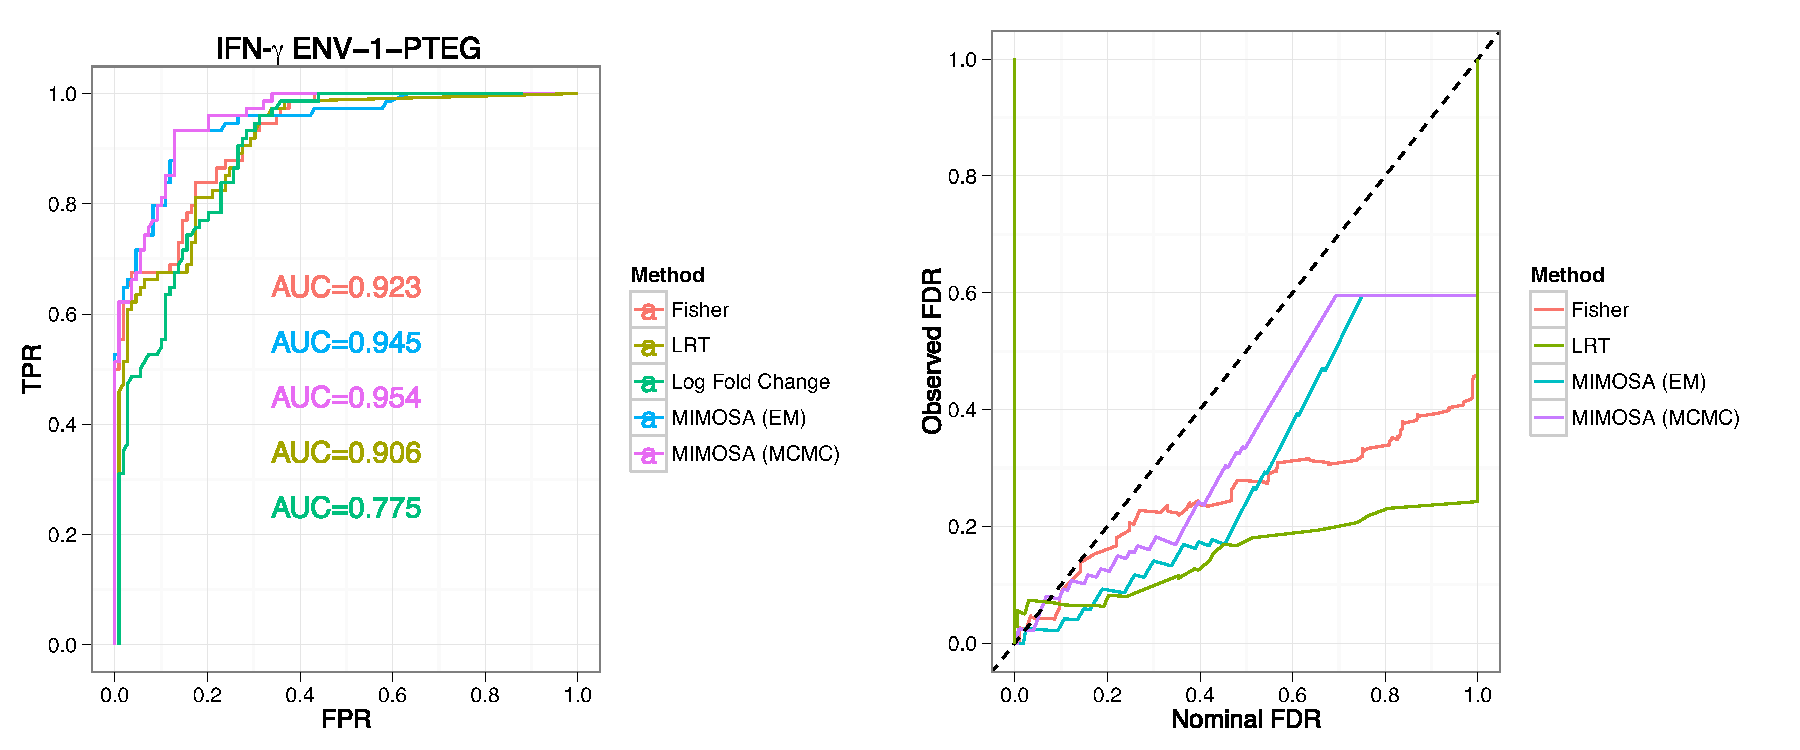
\includegraphics[width=.75\columnwidth]{Figures/2}\\ 
%   \includegraphics[width=.75\columnwidth]{Figures/12} 
\begin{tikzpicture}
    \node[anchor=south west,inner sep=0] at (0,0) {\includegraphics[width=.5\columnwidth]{Figures/12}};
    \node[anchor=south west, inner sep=0] at (8,0){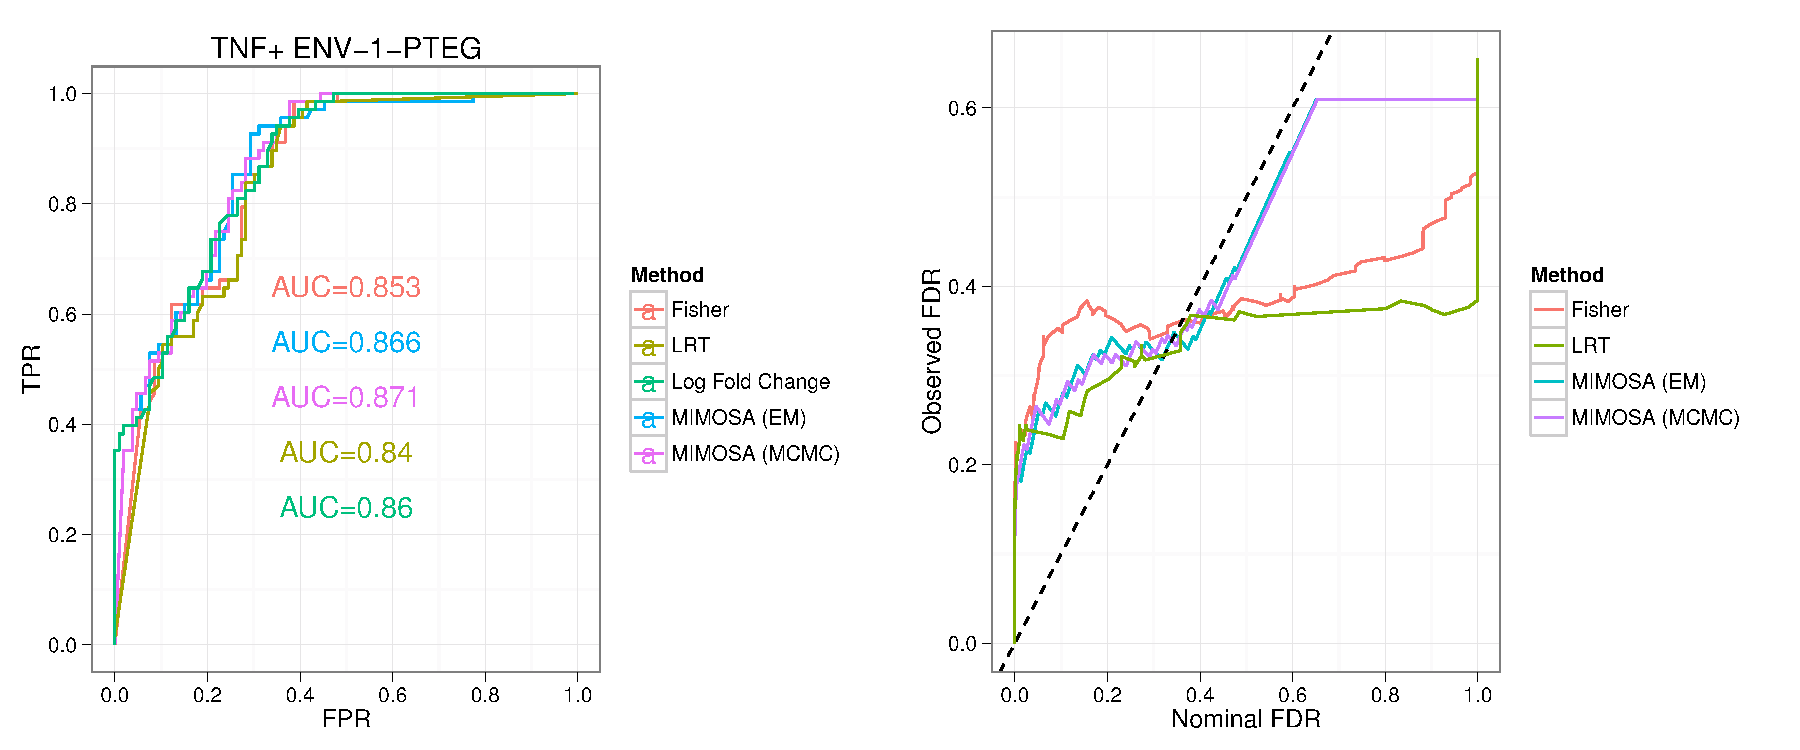
\includegraphics[width=.5\columnwidth]{Figures/3}};
    \node[anchor=south west, inner sep=0] at (0,-3.75){\includegraphics[width=.5\columnwidth]{Figures/5}};
    \node[anchor=south west, inner sep=0] at (8,-3.75){\includegraphics[width=.5\columnwidth]{Figures/6}};
    \node[anchor=south west, inner sep=0] at (0,-7.5){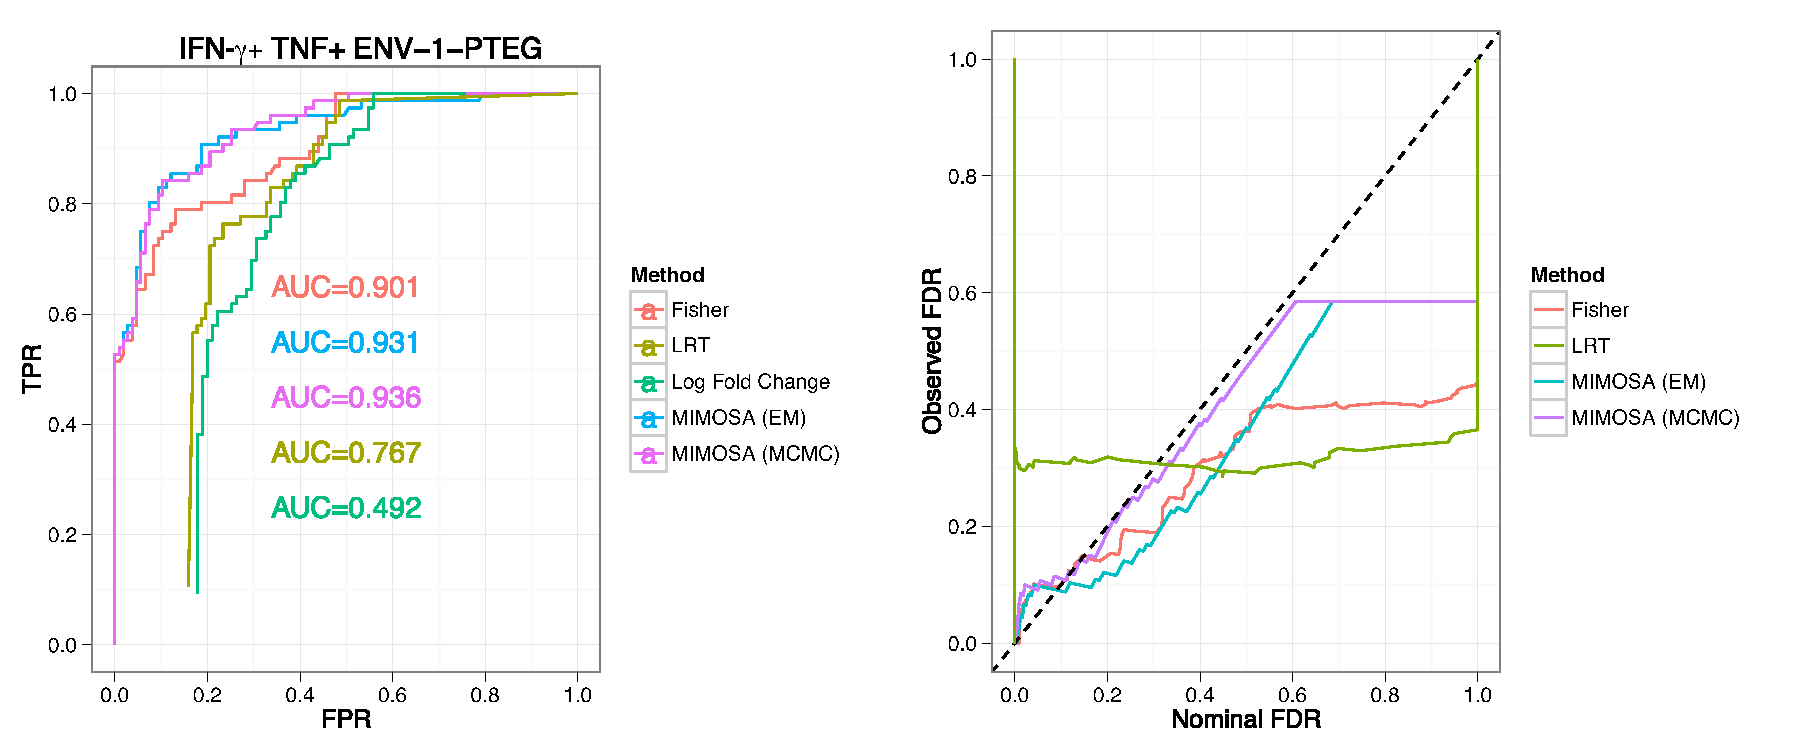
\includegraphics[width=.5\columnwidth]{Figures/7}};
    \node[anchor=south west, inner sep=0] at (8,-7.5){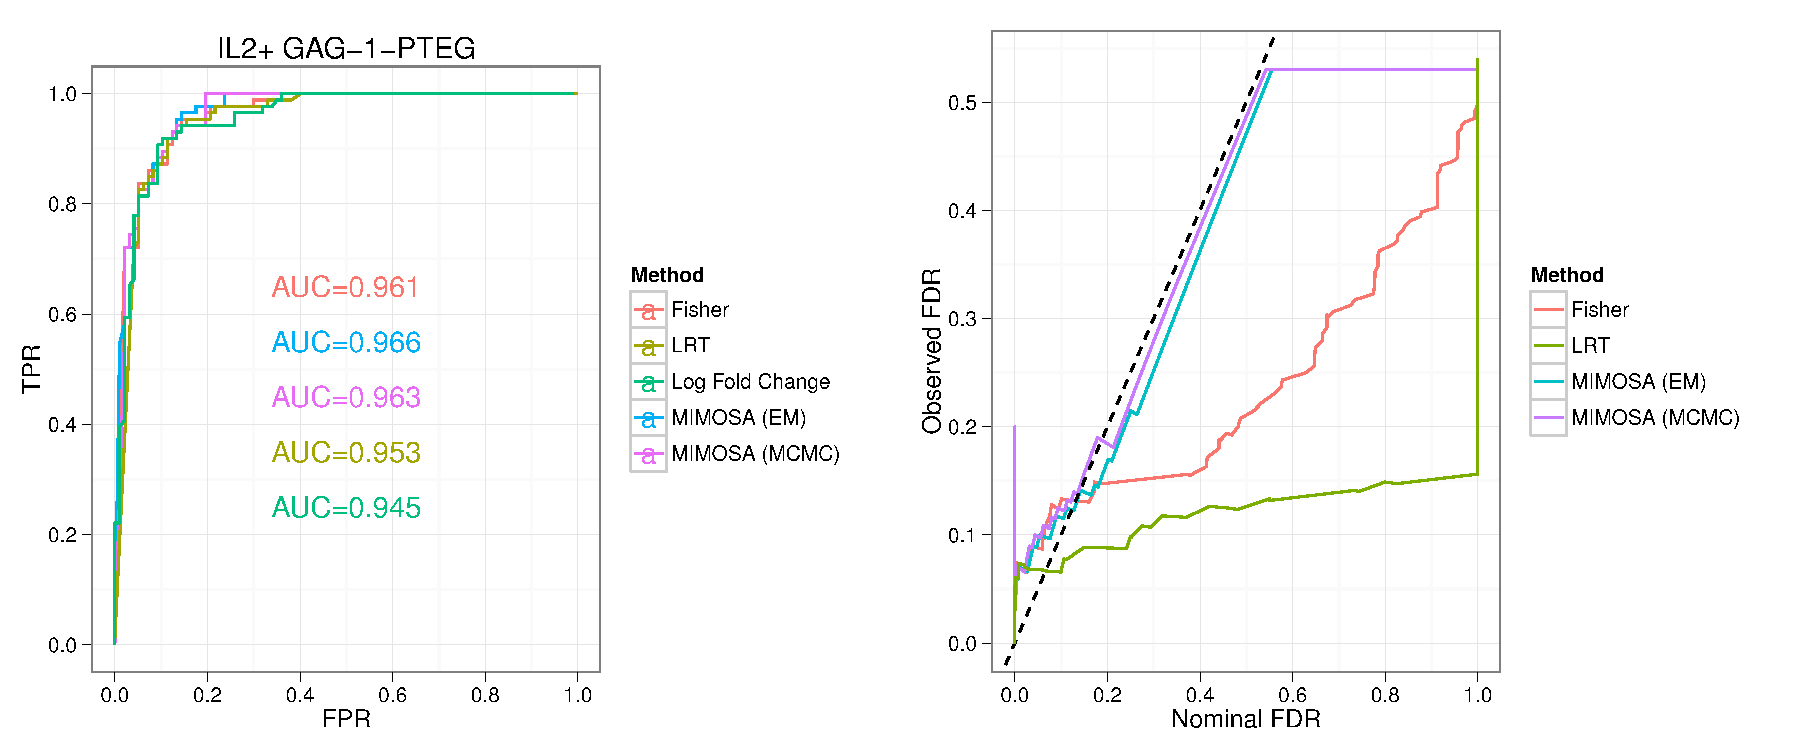
\includegraphics[width=.5\columnwidth]{Figures/8}};
    \node[anchor=south west, inner sep=0] at (0,-11.25){\includegraphics[width=.5\columnwidth]{Figures/9}};
    \node[anchor=south west, inner sep=0] at (8,-11.25){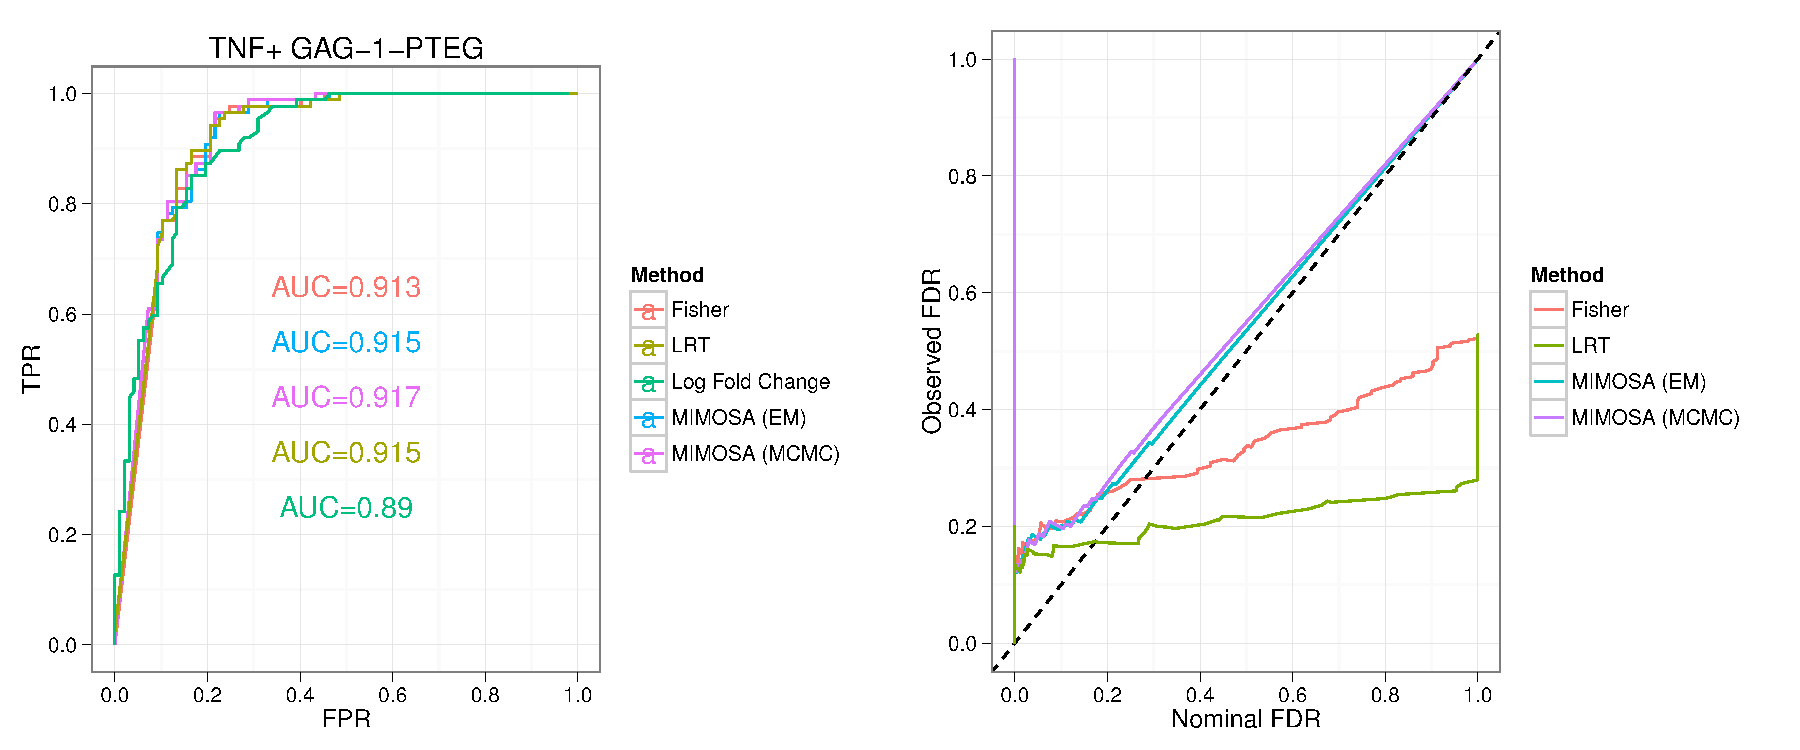
\includegraphics[width=.5\columnwidth]{Figures/10}};
    \node[anchor=south west, inner sep=0] at (0,-15){\includegraphics[width=.5\columnwidth]{Figures/11}};
    \node[anchor=south west, inner sep=0] at (8,-15){\includegraphics[width=.5\columnwidth]{Figures/13}};

    \node at (0,3.4) [font=\tiny\sffamily] {A} ;
    \node at (8,3.4) [font=\tiny\sffamily] {B} ;
    \node at (0,-0.5) [font=\tiny\sffamily] {C} ;
    \node at (8,-0.5) [font=\tiny\sffamily] {D} ;
    \node at (0,-4) [font=\tiny\sffamily] {E} ;
    \node at (8,-4) [font=\tiny\sffamily] {F} ;
    \node at (0,-7.75) [font=\tiny\sffamily] {G} ;
    \node at (8,-7.75) [font=\tiny\sffamily] {H} ;
    \node at (0,-11.75) [font=\tiny\sffamily] {I} ;
    \node at (8,-11.75) [font=\tiny\sffamily] {J} ;
    \end{tikzpicture}
   \caption{Comparison of MIMOSA on other cytokines and cytokine combinations for ENV-1-PTEG and GAG-1-PTEG stimulated CD4+ T-cells from the HVTN065 trial.}
\label{fig:HVTN065Results}
\end{figure}

\begin{figure}[htbp] %  figure placement: here, top, bottom, or page
   \centering
%   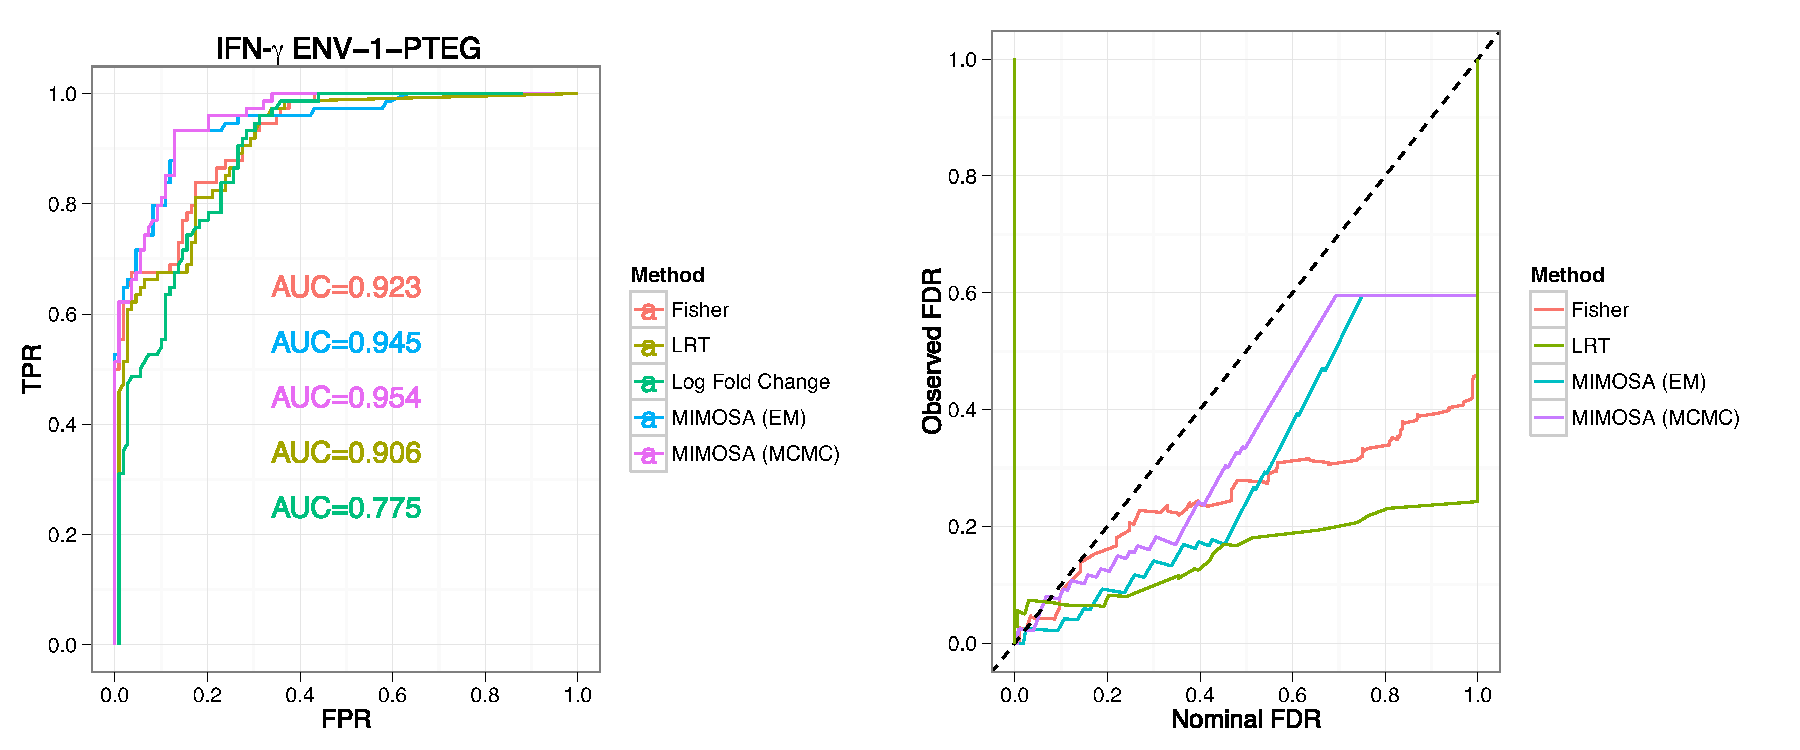
\includegraphics[width=.75\columnwidth]{Figures/2}\\ 
%   \includegraphics[width=.75\columnwidth]{Figures/12} 
\begin{tikzpicture}
    \node[anchor=south west, inner sep=0] at (0,0){\includegraphics[width=.5\columnwidth]{Figures/14}};
    \node[anchor=south west, inner sep=0] at (8,0){\includegraphics[width=.5\columnwidth]{Figures/15}};
    \node[anchor=south west, inner sep=0] at (0,-3.75){\includegraphics[width=.5\columnwidth]{Figures/16}};


    \node at (0,3.4) [font=\tiny\sffamily] {A} ;
    \node at (8,3.4) [font=\tiny\sffamily] {B} ;
    \node at (0,-0.5) [font=\tiny\sffamily] {C} ;
    \end{tikzpicture}
   \caption{Comparison of MIMOSA on other cytokines and cytokine combinations for ENV-1-PTEG and GAG-1-PTEG stimulated CD4+ T-cells from the HVTN065 trial.}
\label{fig:HVTN065ResultsCont}
\end{figure}

\begin{figure}[htbp] %  figure placement: here, top, bottom, or page
   \centering
\begin{tikzpicture}
    \node[anchor=south west,inner sep=0] at (0,0) {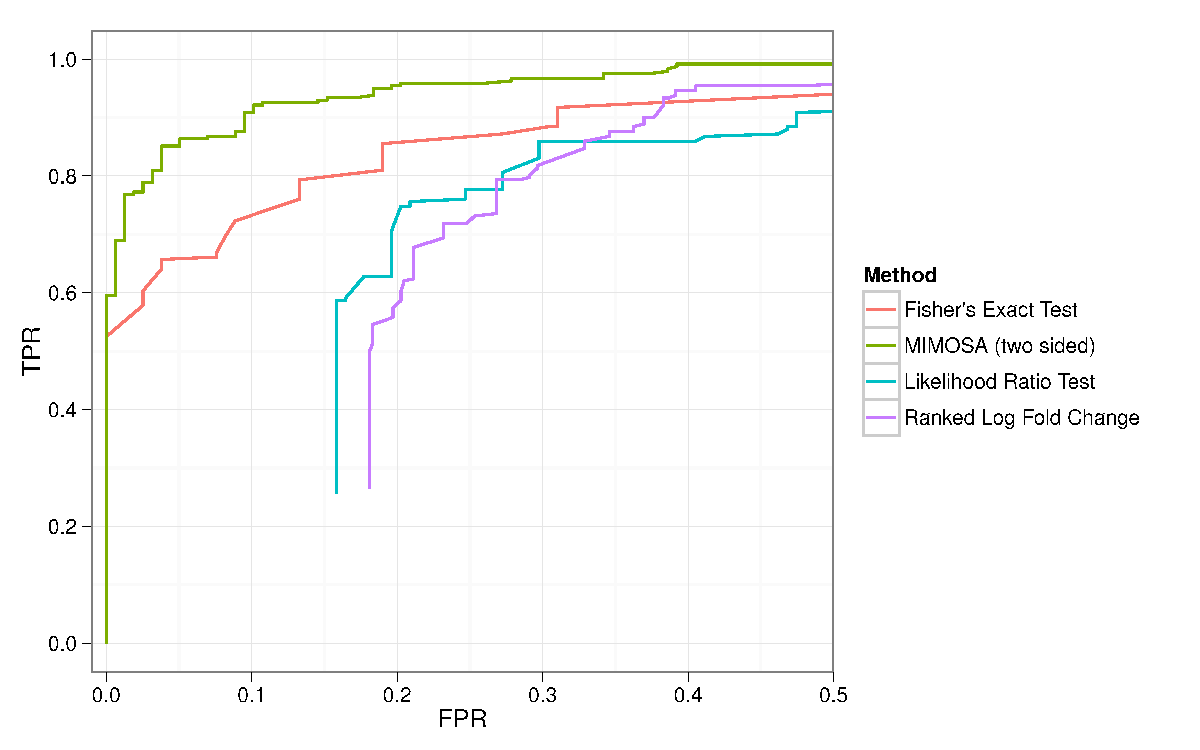
\includegraphics[width=0.4\columnwidth]{Figures/Sim_Truncated_ROC_5000.pdf}};
    \node[anchor=south west, inner sep=0] at (6,0) {\includegraphics[width=0.4\columnwidth]{Figures/Sim_Truncated_FDR_5000.pdf}};
    \node at (0,3.4) [font=\tiny\sffamily] {A} ;
    \node at (4.6,3.4) [font=\tiny\sffamily] {B} ;
 \end{tikzpicture}
   \caption{Unconstrained MIMOSA model fit to data where model assumptions are violated. Two--sided data were simulated from a model where the proportions were drawn from a truncated normal distribution over $[0,1]$, rather than a Beta distribution. A) Average ROC curves from 10 simulations and B) average observed vs nominal FDR from 10 simulations at N=5,000.}
   \label{fig:simulations_trunc}
\end{figure}

%\section{Data Import, Preprocessing, and Gating}
%The ICS assay data was imported into R from the original flowJo workspaces (version 6, TreeStar Inc, Ashland, OR)  using the BioConductor tool, \textit{flowWorkspace} (v 1.1.6) and ncdfFlow (v 1.1.4). Data were preprocessed using the flowJo--defined compensation matrices and data transformations extracted from the workspace file, and gated using methods from the flowCore package (v 1.19.2) to extract counts of cytokine positive and negative T--cells for each sample and stimulation~\cite{Hahne:2009vv}.

%\section{Statistical Analysis in the Published Trial}
%\label{supp:statpublished}
%The methodology for statistical analysis and calling responders and non--responders in the original vaccine trial is described in the original publication~\cite{Peiperl:2010ej}. In general, a participant is called a ``responder'' to an antigen stimulation if, for a given cytokine, the number of cytokine--positive T-cells in the antigen--stimulated sample is significantly greater (for some statistical measure of significance) than the number of cytokine--positive T-cells for the negative control (unstimulated) sample from the same individual. In the original trial, significance was measured via one--sided Fisher's exact test for each participant and cytokine, comparing stimulated against unstimulated samples from that individual. In order to control the false positive rate for responder calls, made based on positivity for multiple cytokines, a discrete Bonferroni adjustment for multiple comparisons (across cytokines) was applied, and stimulations with an adjusted p--value below $\alpha = 0.00001$ were called positive~\cite{Horton:2007tsa}. 

%\subsection{Derivation of the Beta--Binomial Model for $p_s=p_u$ and $p_s>p_u$}
%\label{sec:derivation}
%
%We derive the posterior predictive distribution and marginal log--likelihood for the null model ($p_s=p_u$) and the alternative model ($p_s>p_u$) below: patient indices, $i$ on the $\left<N_s,n_s,N_u,n_u\right>$ are omitted for clarity. 
%For model \eqref{eq:null}, ($p_s=p_u, \alpha_s=\alpha_u, \beta_s=\beta_u$), the posterior predictive distribution of the data given the model is:
% \begin{align}
% 	\mathrm{Pr}(y_i|\alpha_u,\beta_u) &= \int\limits_{p_u=0}\limits^{1} \mathrm{Pr}(y_i,p_u|\alpha_u,\beta_u)dp_u\\
%	&=\int\limits_{p_u=0}\limits^{1} \mathrm{Pr}(y_i|p_u)\mathrm{Pr}(p_u|\alpha_u,\beta_u)dp_u\\
%	\begin{split}
%		=\int\limits_{p_u=0}\limits^{1}\binom{N_s+n_s}{n_s}p_u^{n_s}(1-p_u)^{N_s}\binom{N_u+n_u}{n_u}p_u^{n_u}(1-p_u)^{N_u}\cdot \\ 
%		\frac{1}{\mathrm{B}(\alpha_u,\beta_u)}p_u^{\alpha_u-1}(1-p_u)^{\beta_u-1}dp_u
%	 \end{split}\\
%	 \begin{split}
% 	=\binom{N_s+n_s}{n_s}\binom{N_u+n_u}{n_u}\frac{1}{\mathrm{B}(\alpha_u,\beta_u)}\cdot\\ \int\limits_{p_u=0}\limits^{1}p_u^{n_s+n_u+\alpha_u-1}(1-p_u)^{N_s+N_u+\beta_u-1}dp_u
%	\end{split}\\
%	\intertext{The integrand is the kernel of a beta distribution with parameters $\left(n_u+n_s+\alpha_u,N_u+N_s+\beta_u\right)$, giving a closed form expression for the  posterior predictive distribution of model \eqref{eq:null}:}
%	\mathrm{Pr}(y_i|\alpha_u,\beta_u)&=\binom{N_s+n_s}{n_s}\binom{N_u+n_u}{n_u}\frac{\mathrm{B}(n_s+n_u+\alpha_u,N_s+N_u+\beta_u)}{\mathrm{B}(\alpha_u,\beta_u)}\label{eq:model1postsupp}\\
%	\intertext{with marginal log--likelihood:}
%	\begin{split}
%	\mathcal{L}(\alpha_u,\beta_u|\mathbf{y})=\sum_{i=1}^P\left[\log{\binom{N^i_{s}+n^i_{s}}{n^i_{s}}}+\log{\binom{N^i_{u}+n^i_{u}}{n^i_{u}}}+\right.\\
%	\left.\log{\left(\mathrm{B}(n^i_s+n^i_u+\alpha_u,N^i_s+N^i_u+\beta_u)\right)}\right]-P\log\left(\mathrm{B}(\alpha_u,\beta_u)\right)\label{eq:model1MLLsupp}
%	\end{split}
% \end{align} 
% 
%For model \eqref{eq:alternate}, ($p_s>p_u$), the posterior predictive distribution of the data given the model is:
%\begin{align}
% 	\mathrm{Pr}(y_i|\alpha_u,\beta_u,\alpha_s,\beta_s) &= \int\limits_{p_u=0}\limits^1\int\limits_{p_s>p_u}\limits^{1} \mathrm{Pr}(y_i,p_u,p_s|\alpha_u,\beta_u,\alpha_s,\beta_s) dp_u  dp_s\label{eq:postpredmodel2}\\
%	\intertext{Assuming independence of stimulated and unstimulated observations in \eqref{eq:postpredmodel2}:} 
%	&=\int\limits_{p_u=0}\limits^{1}\int\limits_{p_s>p_u}\limits^1 \mathrm{Pr}(n_s|p_s)\mathrm{Pr}(n_u|p_u)\mathrm{Pr}(p_u|\alpha_u,\beta_u)\mathrm{Pr}(p_s|\alpha_s,\beta_s)dp_u dp_s\\
%		&=\int\limits_{p_u=0}\limits^{1}\mathrm{Pr}(n_u|p_u)\mathrm{Pr}(p_u|\alpha_u,\beta_u)dp_u \int\limits_{p_s>p_u}\limits^1 \mathrm{Pr}(n_s|p_s)\mathrm{Pr}(p_s|\alpha_s,\beta_s)dp_s\\
%		\begin{split}
%	=\int\limits_{p_u=0}\limits^{1}\left[ \binom{N_u+n_u}{n_u}p_u^{n_u}(1-p_u)^{N_u} \frac{1}{\mathrm{B}(\alpha_u,\beta_u)}p_u^{\alpha_u-1}(1-p_u)^{\beta_u-1}d p_u\right]\cdot \\ \int\limits_{p_s>p_u}\limits^{1}\left[ \binom{N_s+n_s}{n_s}p_s^{n_s}(1-p_s)^{N_s} \frac{1}{\mathrm{B}(\alpha_s,\beta_s)}p_s^{\alpha_s-1}(1-p_s)^{\beta_s-1}d p_s\right]
%	\end{split}\\
%	\begin{split}
%	 =\binom{N_u+n_u}{n_u} \binom{N_s+n_s}{n_s}\frac{1}{\mathrm{B}(\alpha_u,\beta_u)}\frac{1}{\mathrm{B}(\alpha_s,\beta_s)}\cdot\\
%	 \int\limits_{p_u=0}\limits^{1}\left[p_u^{n_u+\alpha_u-1}(1-p_u)^{N_u+\beta_u-1} d p_u\right]\int\limits_{p_s>p_u}\limits^{1}\left[p_s^{n_s+\alpha_s-1}(1-p_s)^{N_s+\beta_s-1}d p_s\right]
%	\end{split}
%	\end{align}
%	\begin{align}
%	\begin{split}
%	 =\binom{N_u+n_u}{n_u} \binom{N_s+n_s}{n_s}\frac{1}{\mathrm{B}(\alpha_u,\beta_u)}\frac{1}{\mathrm{B}(\alpha_s,\beta_s)}\cdot\\
%	 \int\limits_{p_u=0}\limits^{1}\left[p_u^{n_u+\alpha_u-1}(1-p_u)^{N_u+\beta_u-1}d p_u \right]\left(1-\int\limits^{p_u}\limits_{p_s=0}\left[p_s^{n_s+\alpha_s-1}(1-p_s)^{N_s+\beta_s-1}d p_s\right]\right)
%	\end{split}
%	\intertext{The second integral can be expressed as the CDF of the beta distribution, also known as the regularized incomplete beta function, $\mathrm{I}_x(\alpha,\beta)$}
%	\begin{split}
%	 =\binom{N_u+n_u}{n_u} \binom{N_s+n_s}{n_s}\frac{1}{\mathrm{B}(\alpha_u,\beta_u)}\frac{\mathrm{B}(n_s+\alpha_s,N_s+\beta_s)}{\mathrm{B}(\alpha_s,\beta_s)}\cdot\\
%	 \int\limits_{p_u=0}\limits^{1}\left[p_u^{n_u+\alpha_u-1}(1-p_u)^{N_u+\beta_u-1} \right]\left(1-\mathrm{I_{p_s}}(n_s+\alpha_s,N_s+\beta_s)\right)d p_u
%	\end{split}\\
%	\intertext{giving the posterior predictive distribution of model \eqref{eq:alternate}}
%	\begin{split}
%		 =\binom{N_u+n_u}{n_u} \binom{N_s+n_s}{n_s}\frac{\mathrm{B}(n_u+\alpha_u,N_u+\beta_u)}{\mathrm{B}(\alpha_u,\beta_u)}\frac{\mathrm{B}(n_s+\alpha_s,N_s+\beta_s)}{\mathrm{B}(\alpha_s,\beta_s)}\cdot\\
%	 \int\limits_{p_u=0}\limits^{1}\left[\frac{1}{\mathrm{B}(n_u+\alpha_u,N_u+\beta_u)}p_u^{n_u+\alpha_u-1}(1-p_u)^{N_u+\beta_u-1} \right]\left(1-\mathrm{I_{p_u}}(n_s+\alpha_s,N_s+\beta_s)\right)d p_u\label{eq:model2postsupp}
%	\end{split}
%\end{align}
%The integral in equation~\eqref{eq:model2postsupp} is computed numerically. The marginal log--likelihood of model~\eqref{eq:alternate} is then:
%\begin{equation}
%		 \begin{split}
%		 \mathcal{L}(\alpha_s,\alpha_u,\beta_s,\beta_u|\mathbf{y})=-P\log\left(\mathrm{B}(\alpha_u,\beta_u)\right)-P\log\left(\mathrm{B}+(\alpha_s,\beta_s)\right)+\\ \sum_{i=0}^P\left\{\log\binom{N^i_u+n^i_u}{n^i_u}+ \log\binom{N^i_s+n^i_s}{n^i_s}+ \log\left(\mathrm{B}(n^i_u+\alpha_u,N^i_u+\beta_u)\right)+ \log\left(\mathrm{B}(n^i_s+\alpha_s,N^i_s+\beta_s)\right)+\right. \\ \left. \log\left(\hspace{1em}\int\limits_{p_u=0}\limits^{1}\left[\frac{1}{\mathrm{B}(n^i_u+\alpha_u,N^i_u+\beta_u)}p_u^{n^i_u+\alpha_u-1}(1-p_u)^{N^i_u+\beta_u-1} \right]\left(1-\mathrm{I_{p_u}}(n^i_s+\alpha_s,N^i_s+\beta_s)\right)d p_u\right)\right\}\label{eq:model2MLLsupp}
%\end{split}
%\end{equation}
%\subsection{The Beta-Binomial Mixture Model}
%For a given stimulation, not all individuals are expected to exhibit an immune response to that stimulation. Therefore, for a set of ICS data, any single observation, ($n^i_s,n^i_u$) could either be derived from model~\eqref{eq:null}, or from model~\eqref{eq:alternate}. We model this situation explicitly using a mixture--model framework.
\clearpage
\bibliographystyle{unsrtnat}
\bibliography{MIMOSA}

\end{document}  
